\documentclass[hidelinks]{article}
\usepackage[a4paper, total={7in, 10in}]{geometry}
\usepackage[dvipsnames]{xcolor}
\usepackage{amsmath}
\usepackage{tikz}
\usepackage{tkz-euclide}
\usepackage[unicode]{hyperref}
\usepackage[all]{hypcap}
\usepackage{fancyhdr}
\usepackage[UTF8,fontset=fandol]{ctex}

\usetikzlibrary{angles,calc, decorations.pathreplacing}

\definecolor{carminered}{rgb}{1.0, 0.0, 0.22}
\definecolor{capri}{rgb}{0.0, 0.75, 1.0}
\definecolor{brightlavender}{rgb}{0.75, 0.58, 0.89}

\title{\textbf{Project 2: Planet Formation}}
\author{刘任达\\盛文哲\\蒋弘杰}
\date{May 30th, 2025}
\begin{document}
\hypersetup{bookmarksnumbered=true,}
\maketitle
\setcounter{tocdepth}{2}
\begin{Large}
\tableofcontents
\end{Large}%
\pagebreak

\section{背景介绍——太阳系的形成与演化}
有关世界起源和命运的思想可以追溯到已知最早的文字记载。迈向太阳系演化形成理论的第一步是对日心说的广泛认同,现今太阳系形成的标准理论:\textbf{星云假说},从其在18世纪被伊曼纽·斯威登堡、伊曼努尔·康德、和皮埃尔-西蒙·拉普拉斯提出之日起就屡经采纳和摒弃。对该假说重大的批评是它很明显无法解释太阳相对其行星而言缺少角动量。然而,自从1980年代早期对新恒星的研究显示,正如星云假想预测的那样,它们被冷的气体和灰尘的盘环绕着,才导致这一假想的重新被接受。其主要形成过程有以下几个阶段:
\subsection{前太阳星云}
星云假说主张太阳系从一巨大的有几光年跨度的分子云的碎片引力塌陷的过程中形成。几十年前,传统观点还是认为太阳是在相对孤立中形成的,但对古陨石的研究发现短暂的同位素(如铁-60)的踪迹,该元素只能在爆炸及寿命较短的恒星中形成。这显示在太阳形成的过程中附近发生了若干次超新星爆发。其中一颗超新星的冲击波可能在分子云中造成了超密度区域,导致了这个区域塌陷,从而触发了太阳的形成。因为只有大质量、短寿恒星才会产生超新星爆发,太阳一定是在一个产生了大质量恒星的一个大恒星诞生区域里(可能类似于猎户座大星云)形成。

这些被称为“前太阳星云”的塌陷气体区域中的一部分将形成太阳系。这一区域直径在7000到20,000天文单位(AU)其质量刚好超过太阳。它的组成跟今天的太阳差不多。由太初核合成产生的元素氢、氦、和少量的锂组成了塌陷星云质量的98\%。剩下的2\%质量由在前代恒星核合成中产生的金属重元素组成。在这些恒星的晚年它们把这些重元素抛射成为星际物质。

因为角动量守恒,星云塌陷时转动加快。随着星云浓缩,其中的原子相互碰撞频率增高,把它们的动能转化成热能。其质量集中的中心越来越比周边环绕的盘热。大约经过100,000年,在引力、气体压力、磁场力和转动惯量的相互竞争下,收缩的星云扁平化成了一个直径约200AU的\textbf{原行星盘},并在中心形成一个热致密的原恒星(内部氢聚变尚未开始的恒星)。

太阳发展到了这一演化点时,已被认为是一颗金牛T星类型的恒星。对金牛T星的研究表明它们常伴以0.001-0.1太阳质量的前行星物质组成的盘。这些盘伸展达几百AU——哈勃太空望远镜已经观察过在恒星形成区(如猎户座大星云)直径达1000AU的原星盘——并且相当冷,最热只能达到一千开尔文。

在五千万年内,太阳核心的温度和压力变大,大到氢开始聚变,产生内部能源抗拒引力收缩的力直到达至静力平衡[20]。这意味着太阳成为了主序星,这是它生命中的一个主要阶段。主序星从它们核心的氢聚变为氦的过程中产生能量。太阳至今还是一颗主序星。

\subsection{行星的形成}
太阳系里诸多行星均被认为成形于“太阳星云”,而太阳星云是太阳形成中剩下的气体和尘埃形成的圆盘状云。目前被接受的行星形成假说称为\textbf{吸积},在这里行星从绕原恒星的轨道上的尘埃颗粒开始形成。通过直接收缩,这些颗粒形成一到十公里直径的块状物, 然后它们互相碰撞形成更大的尺寸约5公里的天体(\textbf{微行星})。透过进一步相撞逐渐加大它们的尺寸, 在接下来的几百万年中大约每年增加几厘米。

内太阳系(距中心直径4天文单位以内的区域)过于温暖以至于易挥发的如水和甲烷分子难以聚集,所以那里形成的微行星只能由高熔点的物质形成,如铁、镍、铝和石状硅酸盐。这些石质天体会成为类地行星(水星、金星和火星)。这些物质在宇宙中很稀少,大约只占星云质量的0.6\%,所以类地行星不会长得太大。类地行星胚胎在太阳形成100,000年后长到0.05地球质量,然后就停止聚集质量;随后的这些行星大小的天体间的相互撞击与合并使它们这些类地行星长到它们今天的大小。类地行星的成分是太阳核心成分的重要参考。

类木行星(木星、土星、天王星和海王星)形成于更远的冻结线之外,在介于火星和木星轨道之间的物质冷到足以使易挥发的冰状化合物保持固态。类木行星上的冰比类地行星上的金属和硅酸盐更丰富,使得类木行星的质量长得足够大到可以俘获氢和氦这些最轻和最丰富的元素。冻结线以外的微行星在3百万年间聚集了4倍地球的质量。今天,这四个类木行星在所有环绕太阳的天体质量中所占的比例可达99\%。理论学者认为木星处于刚好在冻结线之外的地方并不是偶然的。因为冻结线聚集了大量由向内降落的冰状物质蒸发而来的水,其形成了一个低压区,加速了轨道上环绕的尘埃颗粒的速度阻止了它们向太阳落去的运动。在效果上,冻结线起到了一个壁垒的作用,导致物质在距离太阳约5天文单位处迅速聚集。这些过多的物质聚集成一个大约有10个地球质量的胚胎,然后开始通过吞噬周围星盘的氢而迅速增长,只用了1000年就达到150倍地球质量并最终达到318倍地球质量。土星质量显著地小可能是因为它比木星晚了几百万年形成,当时所能使用的气体少了。

\subsection{后续演化}
行星原先被认为是在我们今天看到的它们的轨道内或附近形成的。但这一观点在20世纪晚期和21世纪初期发生了巨变。现在认为太阳系在最初形成之后看上去跟现在很不一样:在内太阳系有几个至少跟金星一样大的天体,外太阳系也比现在紧密,柯伊伯带离太阳要近得多。

\subsubsection{类地行星}
类地行星的成分被学者认为与太阳核心的成分存在高度相关性,行星形成时代结束后内太阳系有50-100个月球到火星大小的行星胚胎。进一步的生长可能只是由于这些天体的相互碰撞和合并,这一过程持续了大约1亿年。这些天体互相产生引力作用,互相拖动对方的轨道直到它们相撞,长得更大,直到最后我们今天所知的4个类地行星初具雏形。其中的一个这样的巨大碰撞据信导致了月球的形成, 另外一次剥去了早期水星的外壳。

此模型未解决的问题是它不能解释这些原类地行星的初始轨道——得要相当的偏心圆形才能相撞——是如何形成今天这样相当稳定且接近圆形的轨道的。此“偏圆去除”的假说之一认为在气体盘中形成的类地行星尚未被太阳驱离。这些残余气体的“引力拖拉”终将降低行星的能量,平滑化它们的轨道。不过,如果存在这样的气体,一开始它就会防止类地行星的轨道变得如此偏圆。另一个假说认为引力拖拉不是发生在行星和气体之间,而是发生在行星和余留的小天体之间。当大的天体行经小天体群时,小天体受到大天体的引力吸引,在大天体的路径形成了一个高密度区,一个“引力唤醒”,由此降低了大天体使其进入一个更正规的轨道.
\subsubsection{小行星带}
小行星带位于类地行星区外围边缘,离太阳2到4个AU。小行星带开始有多于足以形成超过2到3个地球一样的行星的物质,并且实际上,有很多微行星在那里形成。如同类地行星,这一区域的微行星后来合并形成20到30个月亮到火星大小的行星胚胎;但是因为在木星附近,意味着太阳形成3百万年后这一区域的历史发生了巨大变化。木星和土星的轨道共振对小行星带特别强烈,并且与更多的大质量的行星胚胎的引力交互作用使更多的微行星散布到这些共振中,造成它们在与其他天体碰撞后被撕碎,而不是凝结聚合下去。随着木星在形成后的向内迁移,共振将横扫整个小行星带,动态地激发这一区域的天体数量,并加大它们之间的相对速度。共振和行星胚胎的累加作用要么使微行星脱离小行星带,要么激发它们的轨道倾角和偏心率变化。某些大质量的行星胚胎也被木星抛出,而其它的可能迁移到了内太阳系里,并在类地行星的最终聚集中发挥了作用。 在这个初始消竭时期,大行星和行星胚胎的作用下在小行星带剩下的主要由微行星组成的总质量不到地球的1\%。这仍是目前在主带的质量的10到20倍,约1/2000地球质量。第二消竭阶段据信是当木星和土星进入临时2:1轨道共振时发生,使小行星带的质量下降接近至目前规模。

内太阳系的巨大撞击期可能对地球从小行星带获取其目前的水成分( ~6×1021 公斤)起到了一定的作用。水太易挥发,不会在地球的形成时期就存在,一定是其后从太阳系外部较冷的地方送来的。水可能是由被木星甩离小行星带的行星胚胎和小的微行星带过来的。2006年发现的一些主带彗星也被认为可能是地球的水的来源之一。 在相比之下,从柯伊伯带或更远的区域的彗星带来的不过约6\%地球的水。
\subsubsection{行星迁移}
根据星云假说,外层的两个行星处于“错误位置”,至于木星 土星 小行星可看木星大航向模型(Grand Tack) 。天王星和海王星所处的区域的太阳星云的低密度和它们的更长的轨道周期时间使它们的形成看似非常不合理。这两个行星被认为形成于有更多物质的木星和土星的轨道附近,但后来历经几亿年迁移到了它们今天所处的位置。

海王星之外,太阳系延伸到柯伊伯带、黄道离散天体和奥尔特云,这三个稀疏的小冰状天体群落被认为是绝大多数被观测到的彗星的起源地。以它们离太阳的距离,在太阳星云散离前聚集的速度太慢以至于不足以形成行星,所以最开始的星盘缺乏足够的物质密度来形成行星。柯伊伯带处于距离太阳30到55AU的地方,更远的黄道离散天体延展到100AU,而遥远的奥尔特云起始于大约50,000AU的地方。但起初,柯伊伯带离太阳近得多也致密得多,外围边缘离太阳大约30AU。它的内部边缘刚好在天王星和海王星的轨道外,天王星和海王星的轨道在形成的时候离太阳要近得多(可能15-20AU),并且位置相反,天王星离太阳要比海王星更远。

太阳系形成之后,巨大行星的轨道持续缓慢变化,主要是受到它们与剩下的大量的微行星之间的相互作用的影响。过了5亿到6亿年(大约40亿年前)木星和土星进入2:1共振;土星每当木星环绕太阳两周才环绕太阳一周。这一共振对外围行星造成了引力推力,从而让海王星越过天王星的轨道,“耕”入古柯伊伯带。这些行星群把大部分小冰状天体向内部散播,同时它们自己却向外移动。这些微行星继而以类似的方式驱散它们遇到的下一颗行星,把行星的轨道向外移动,它们自己向内移动。这一过程持续到微行星与木星相互作用,木星的强大引力使它们轨道变得高度椭圆,甚至把它们径直抛出太阳系。这使得木星略微向内移动。这些被木星驱散进入高度椭圆轨道的天体形成了奥尔特云;那些被迁移中的海王星驱散程度较轻的天体形成了现在的柯伊伯带和黄道离散天体。此情形可解释现今柯伊伯带和黄道离散天体的低密度。这些被驱散的天体,包括冥王星,开始被海王星引力束缚,被拉入轨道共振。最终,在微行星盘里的摩擦力使得天王星和海王星的轨道又变圆了。

与外围行星比,内部行星在太阳系的历史中并未发生显著的迁移,因为它们的轨道在大撞击期保持了稳定。

\subsection{卫星形成}
卫星存在于多数行星和其他太阳系天体周围。这些天然卫星有三个可能的来源机制:

    (1) 从绕行星的星盘(只在大型气体行星的情况下)同时生成
    
    (2) 从撞击的残骸形成(如果有浅角度下足够大的撞击)
    
    (3) 捕获经过的天体
    
木星和土星有几个大型卫星,如木卫一伊俄、木卫二欧罗巴、木卫三盖尼米德和土卫六泰坦,它们来源于环绕这两个行星的星盘,形成的方式大概与这两个行星从环绕太阳的星盘中形成的方式相同。这些卫星的巨大尺寸和它们位于行星的切近揭示了它们的来源,俘获方式是不可能具有这些特性的,而其气态特性又意味着它们不可能从撞击残骸中形成。大型气体行星的外围卫星一般偏小偏心且有任意倾角的轨道,这些都是俘获天体预期会有的特性。大部分这样的卫星沿其主星自转的相反方向绕行。最大的不规则卫星是海王星的卫星海卫一特里顿,它被认为是俘获来的柯伊伯带天体。

太阳系固态天体的卫星来自碰撞和俘获。火星的两个小卫星火卫一佛波斯和火卫二戴摩斯被认为是俘获来的小行星,而月球被认为是形成于一次单独的巨大的斜撞。进行撞击的天体估计可能有接近火星一样的质量,碰撞大约发生在大撞击结束的时期。碰撞把撞击天体的一些幔层撞到了轨道上,聚成了月球。该次撞击可能是形成地球的一系列合并的最后一次。过去曾进一步地推测约火星大小的天体曾形成于地球-太阳拉格朗日点中稳定的一处(L4或L5),而后漂离了它所处的位置。冥王星的卫星卡戎可能也是通过大撞击形成的;冥王星-卡戎和地-月系统是太阳系里仅有“卫星至少占较大天体质量的1\%”中的两例。
\begin{figure}
    \centering
    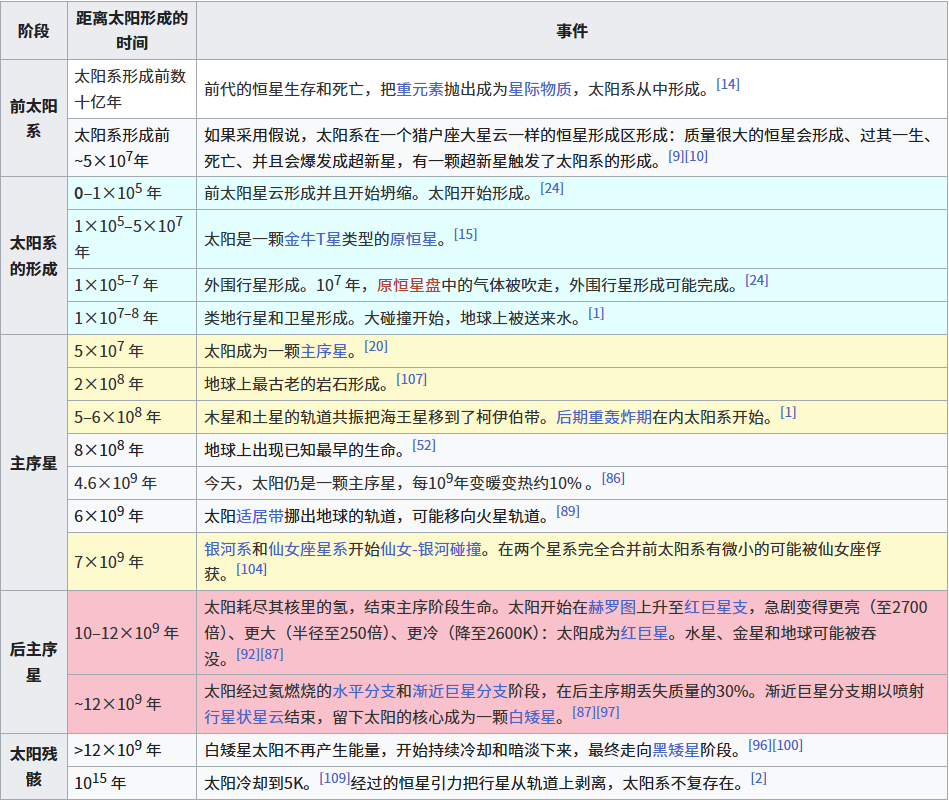
\includegraphics[width=0.5\linewidth]{images/time_list.png}
    \caption{太阳系演化时序表}
    \label{fig:enter-label}
\end{figure}
\section{理论分析}

\section{初步尝试:树算法模拟}
\subsection{一个失败案例}
首先尝试用最直观的方式进行模拟,将太阳静止置于坐标原点,在其周围随机形成一系列小天体,小天体初始速度维持其绕太阳做近似圆周运动,然后通过模拟观察其合并情况。\\

然而,理论估计表明(详细计算可参见3.2节),如果设置小天体质量为$10^{21}$kg量级(约为地球的千分之一),天体的平均间距需要在$10^8$m及以下才能使天体间的相互作用和太阳的潮汐力达到同一量级,然而在$10^{11}$m(一个天文单位)尺度下排布如此之多的点,会带来巨大的演化开销,所以不加任何近似做全局模拟在计算代价上无法接受。\\

因此,我们决定简化模型,在尽可能保留体系和外场性质的条件下,将模拟局限在一个可以接受的区域内,并借小规模模拟的结果来尝试复现行星形成过程中的一些特征。
\subsection{区域和外场设置}
考虑单一质点绕太阳的运动,根据能量守恒和角动量守恒可以得到其运动方程的首次积分如下:
\begin{align*}
    E = &\frac{1}{2}m(\dot{r}^2 + r^2\dot{\theta}^2) - \frac{GMm}{r}\\
    L = &mr^2\dot{\theta}
\end{align*}
其中质点的位置用极坐标$(r,\theta)$描述,$M$和$m$分别代表中心天体和质点的质量,$E$和$L$代表能量和角动量。将切向的部分消去后得到:
$$
E = \frac{1}{2}m\dot{r}^2 + V(r)
$$
其中有效势能$V(r) = - \frac{GMm}{r}+\frac{L^2}{2mr^2}$,由此质点的运动被建模为了一个径向的单自由度问题。\\
在小规模模拟中,为方便起见,将研究的问题设定在二维方形区域上。其中一个方向(记作$x$)和原系统中的径向对应,另一个方向(记作$y$)和原系统中的切向对应。沿$x$方向,假设每个粒子自身绕太阳的运动和小范围的相互作用彼此独立,则有效势场在局部可做二阶展开:
$$
V(r=r_0+x) = -\frac{GMm}{2r_0}+\frac{GMm}{r_0^3}x^2
$$
构成了在$x$方向对粒子的约束,迫使其保持在平衡位置附近。在$y$方向,为了模拟圆环切向的效果,添加周期边界条件,从方形一边离开的粒子会重新从对边进入。\\

从而体系的运动方程为:
\begin{align*}
    m_i\ddot{x_i} = &-\sum_{j\neq i}\frac{Gm_im_j}{r_{ij}^3}x_i-\frac{GMm_i}{r_0^3}(x_i-x_j)\\
    m_i\ddot{y_i} = &-\sum_{j\neq i}\frac{Gm_im_j}{r_{ij}^3}(y_i-y_j)
\end{align*}
其中$r_{ij}=\sqrt{(x_i-x_j)^2+(y_i-y_j)^2}$,$r_0$为一个天文单位,$M$为太阳质量。
\subsection{相互作用的树算法加速}
用有限差分方法求解前述系统涉及到对不同天体间引力的计算,对$N$个粒子逐个计算的复杂度为$\mathcal{O}(N^2)$。对于较大的$N$(如$10^3$量级),这个复杂度会带来过长的模拟用时。为了加速,我们采用Barnes-Hut树算法来加速引力计算,算法流程如下:\\
\\
1. 将区域$[x_{min}, x_{max}]\times[y_{min}, y_{max}]$按中点划分为四叉树;\\
2. 计算每个节点对应区域的尺寸$l$与到目标点的距离$d$,如果$\frac{l}{d}<\theta$(其中$\theta$为某个给定的阈值),按该节点的质心的位置和总质量计算引力,否则对区域进一步划分;\\
3. 直到所有不满足前述条件的区域迭代后均包含不超过一个粒子,停止划分,并计算目标点受到的引力。\\

使用这个算法后,在目标点分布较为均匀时,可以在保持一定精度的基础上使得算法具有$\mathcal{O}(N\log N)$的复杂度,从而使得我们可以在更大的体系中开展实验。
\subsection{天体合并}
在这一部分中,采用最简单的合成判定标准。即假设所有天体均为球形,且其密度为常数$\rho=2.5\times10^3\mathrm{kg}/\mathrm{m}^3$,当两个天体的间距小于它们的半径之和时,发生碰撞,碰撞后所得天体质量为两者之和,速度满足动量守恒定律:
\begin{align*}
    m'&=m_1+m_2\\
    m'\vec{v}&=m_1\vec{v}_1+m_2\vec{v}_2
\end{align*}
\subsection{实验结果}
在3.1节中提到的失败案例如下图所示:
\begin{figure}
    \centering
    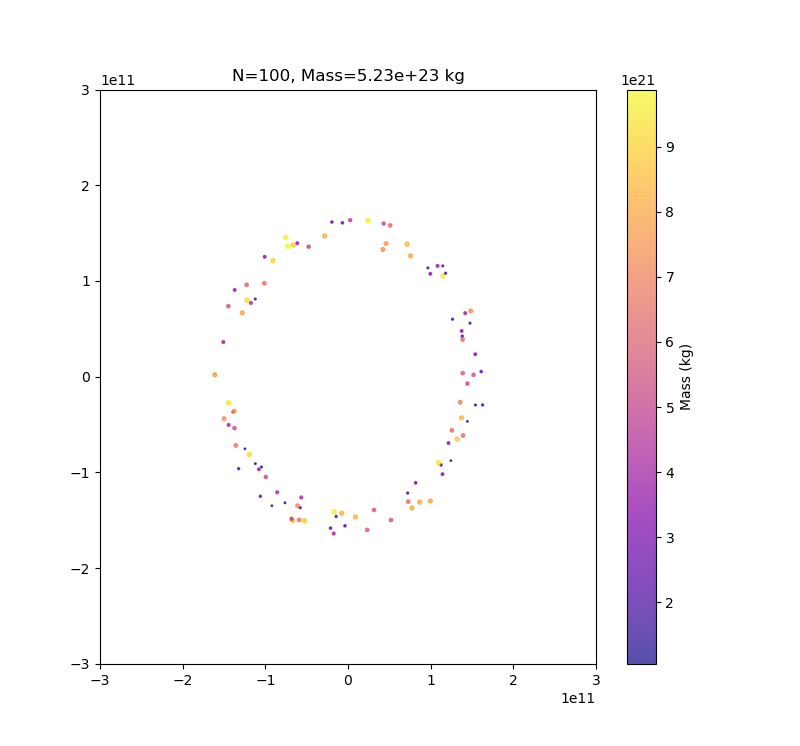
\includegraphics[width=0.5\linewidth]{images/Failure_exp.png}
    \caption{一个失败案例示意图}
\end{figure}
\\

这里粒子所在轨道初始半径在$0.9\sim1.1$个天文单位,实验发现,此时粒子间距过大,以至于在相当长时间内都无法发生合并。\\

换用在3.2节中提出的建模方法后,得到实验结果如下图所示:
\begin{figure}[H]
    \centering
    \subfigure[$N=998$]{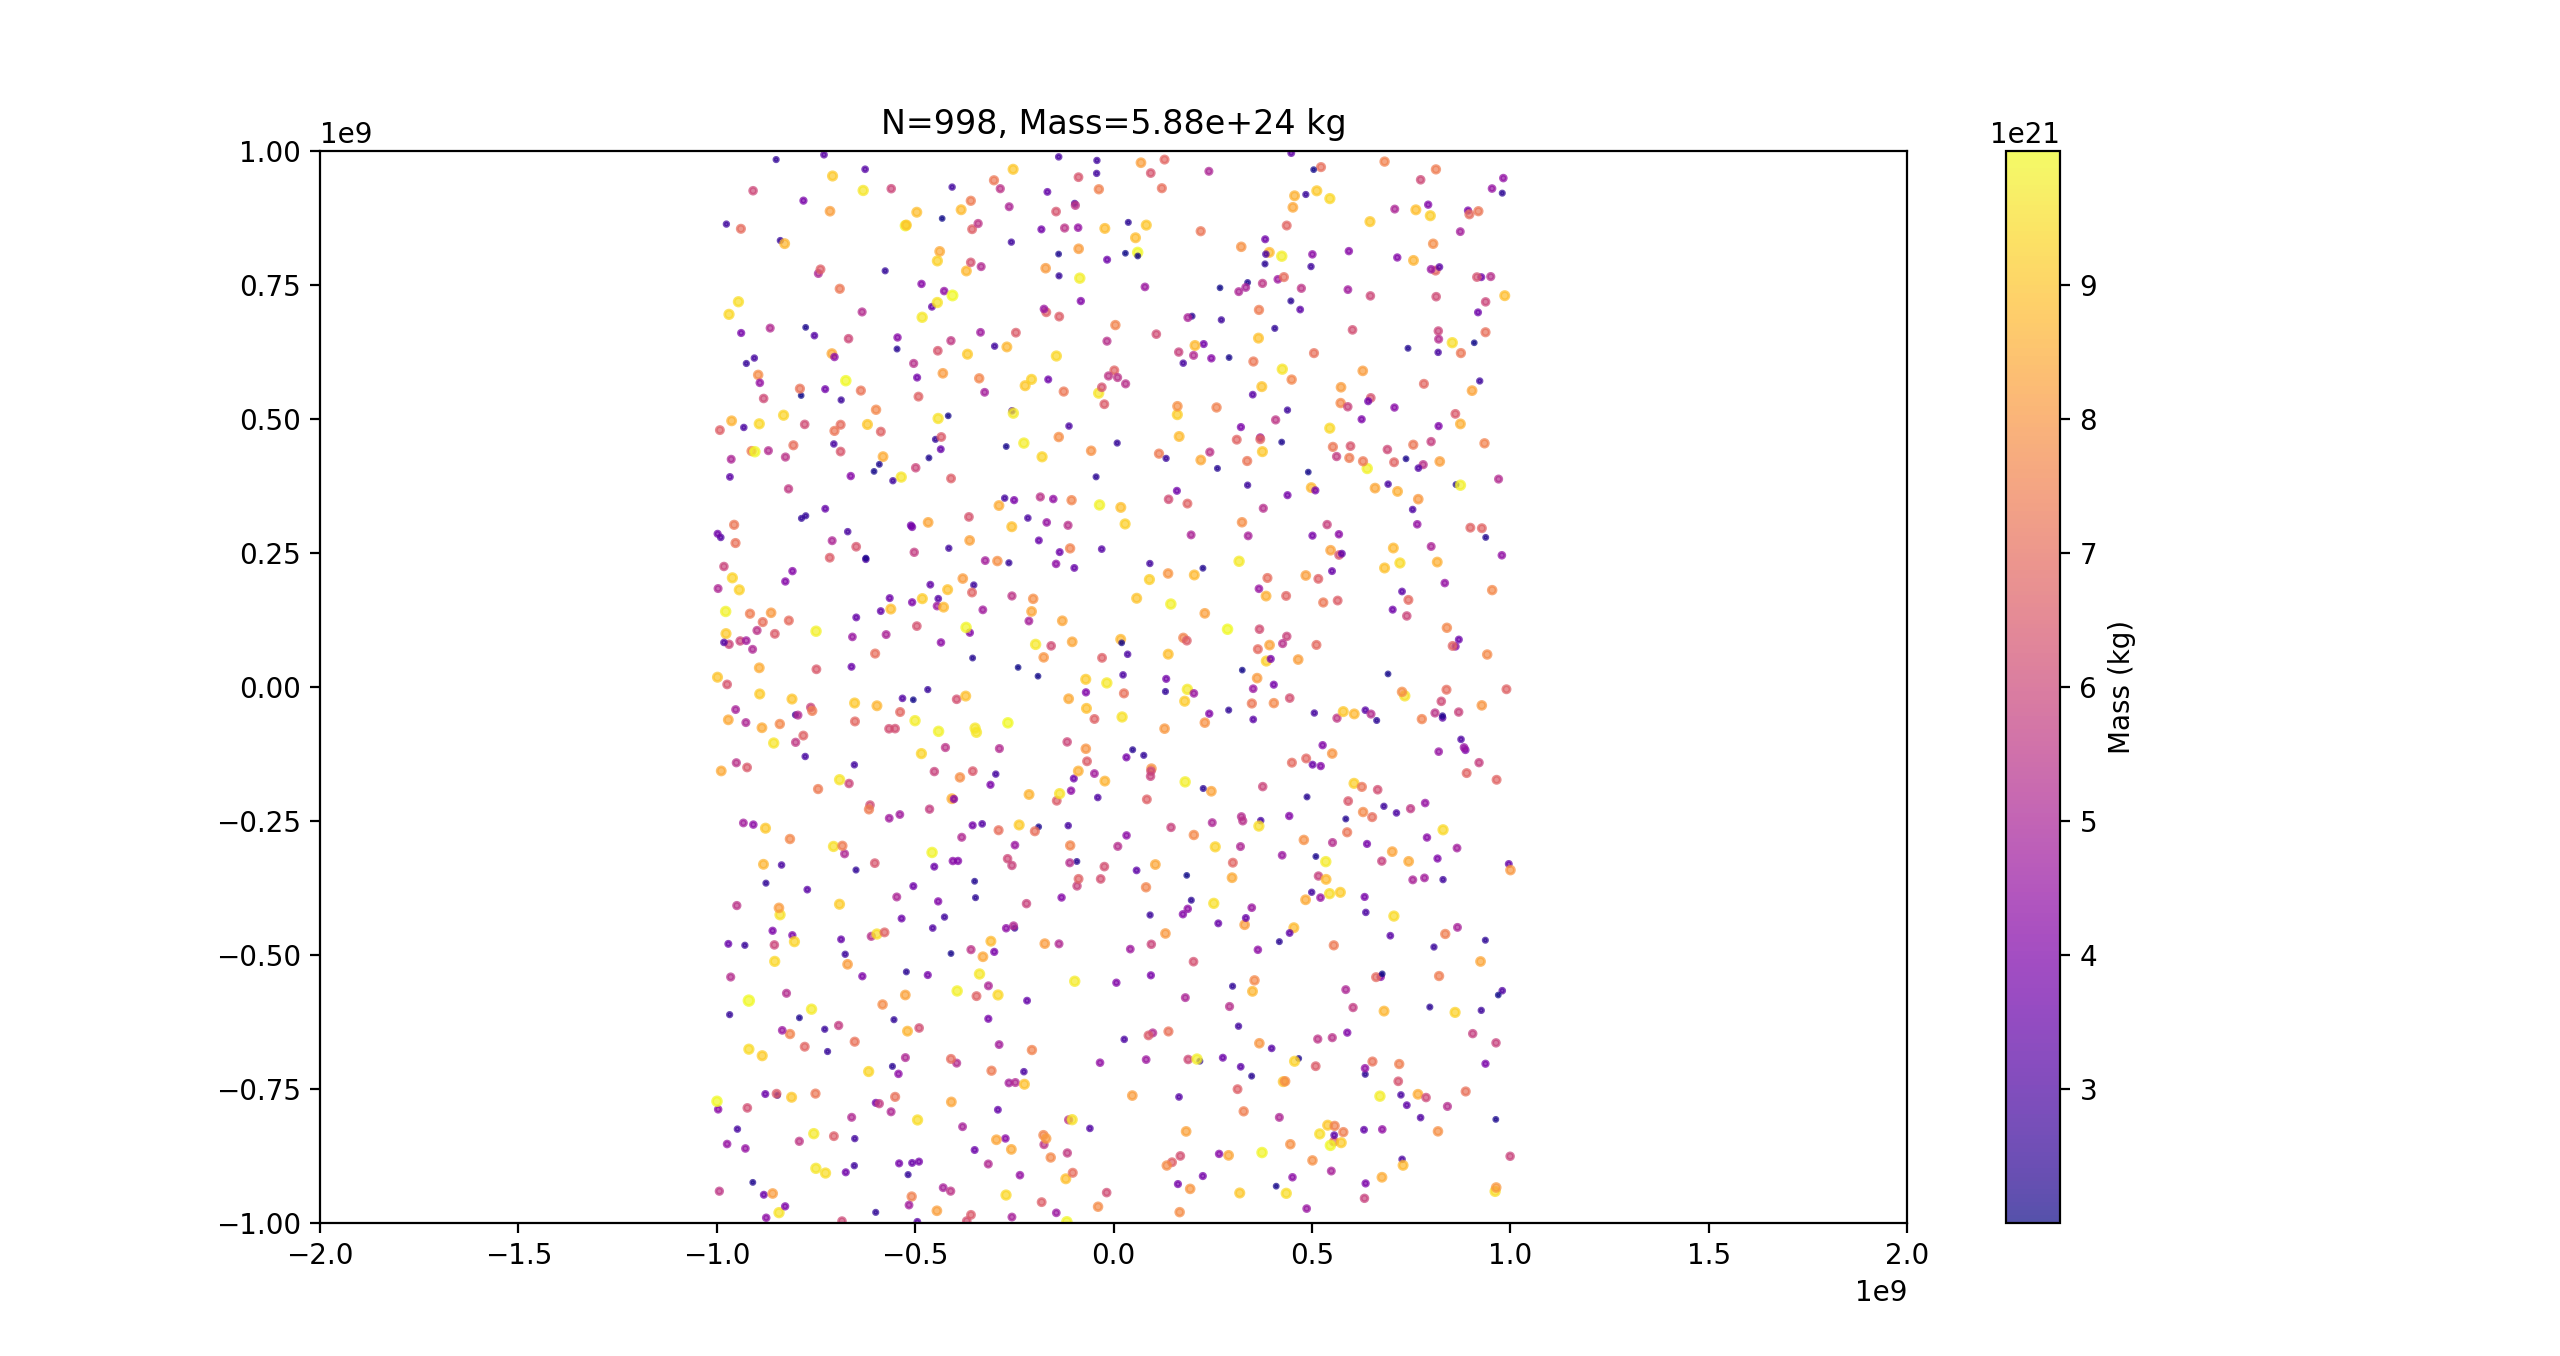
\includegraphics[width=0.48\linewidth]{images/998.png}}
    \subfigure[$N=802$]{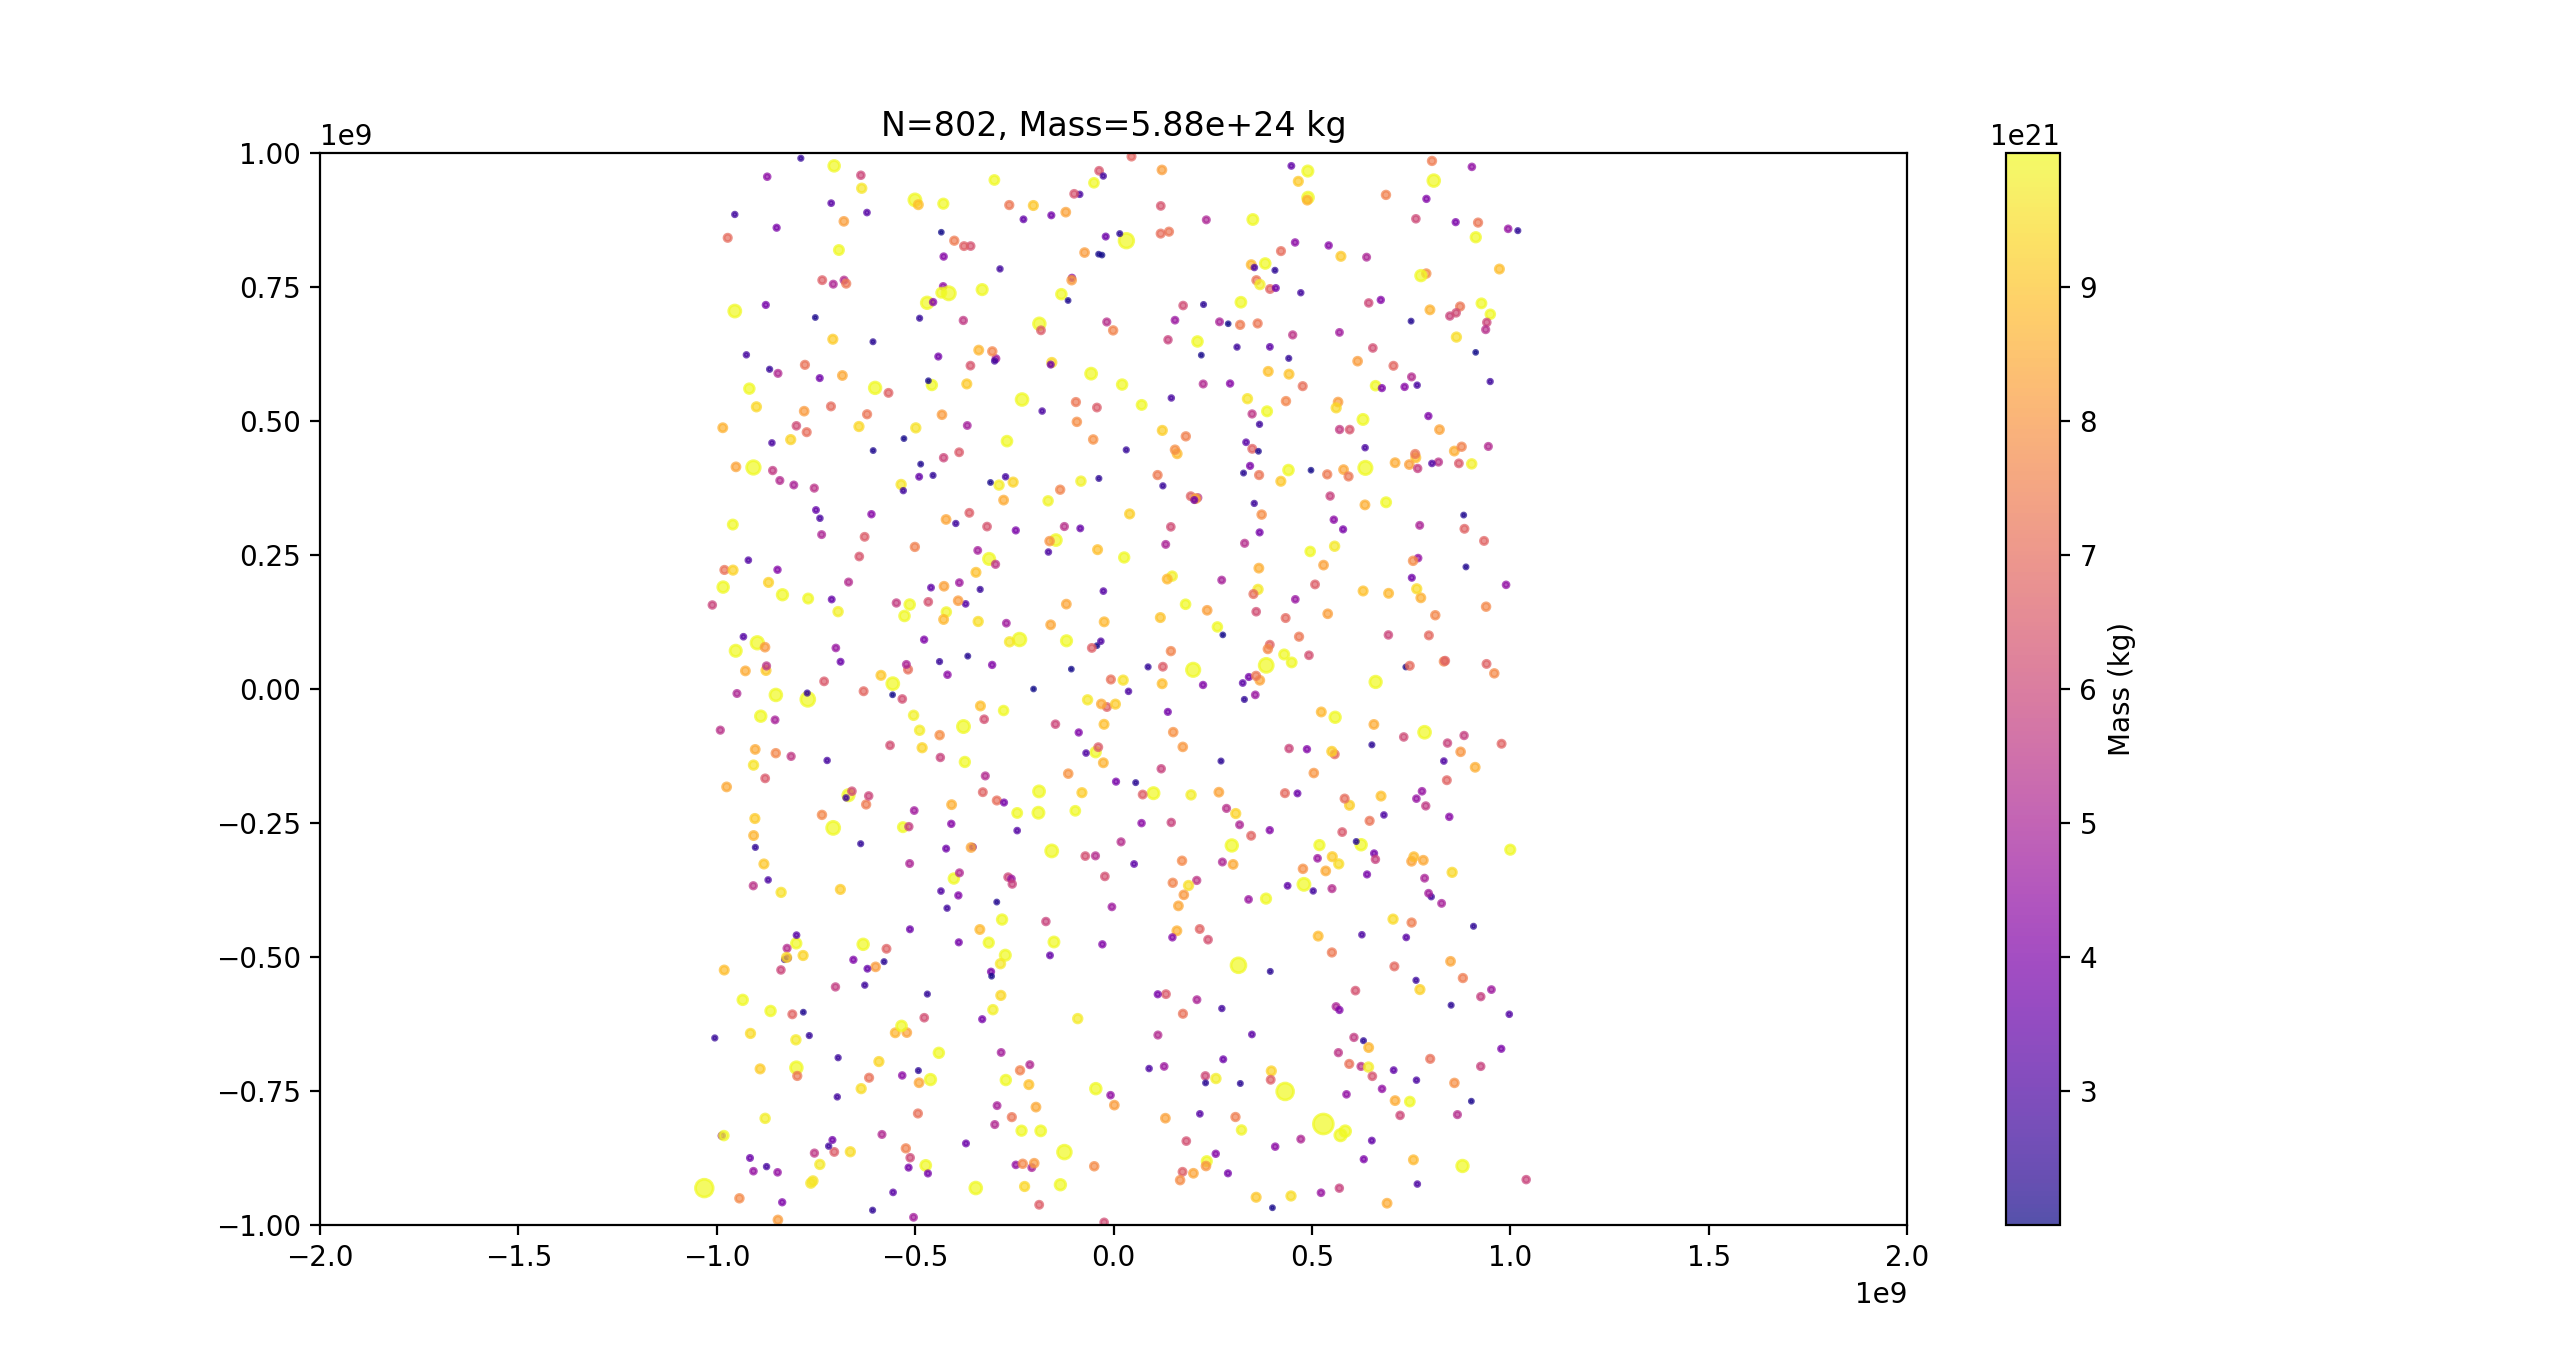
\includegraphics[width=0.48\linewidth]{images/802.png}}
    \subfigure[$N=491$]{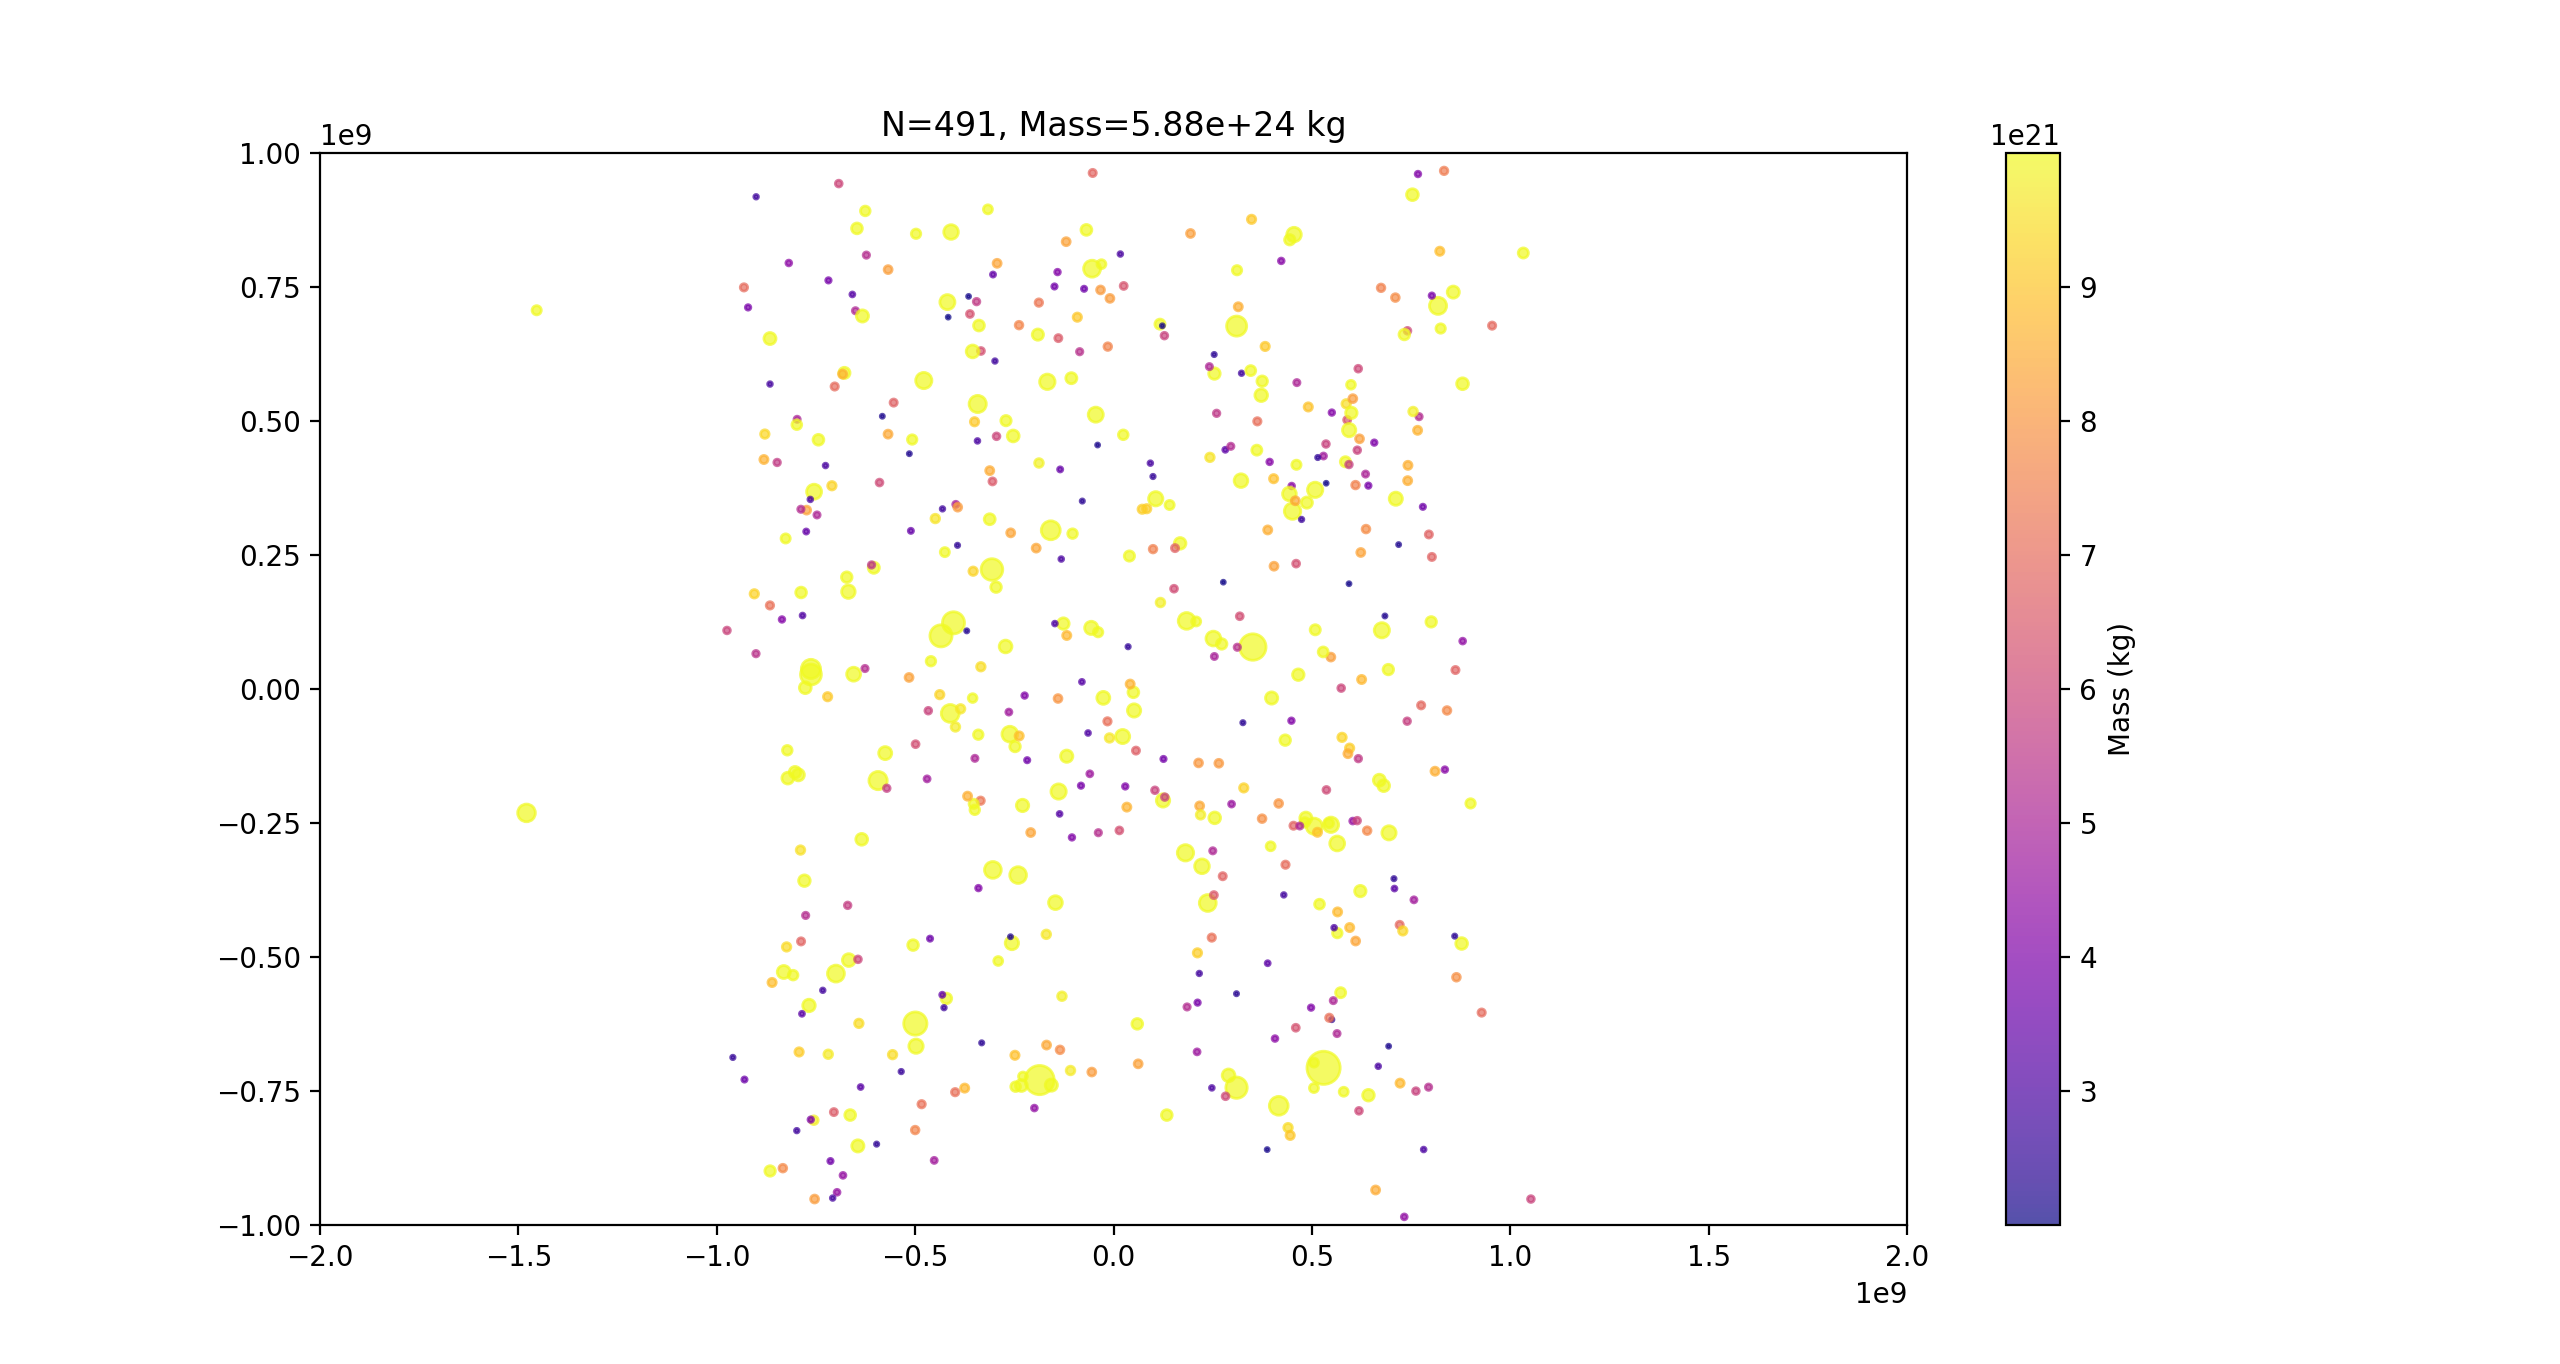
\includegraphics[width=0.48\linewidth]{images/491.png}}
    \subfigure[$N=247$]{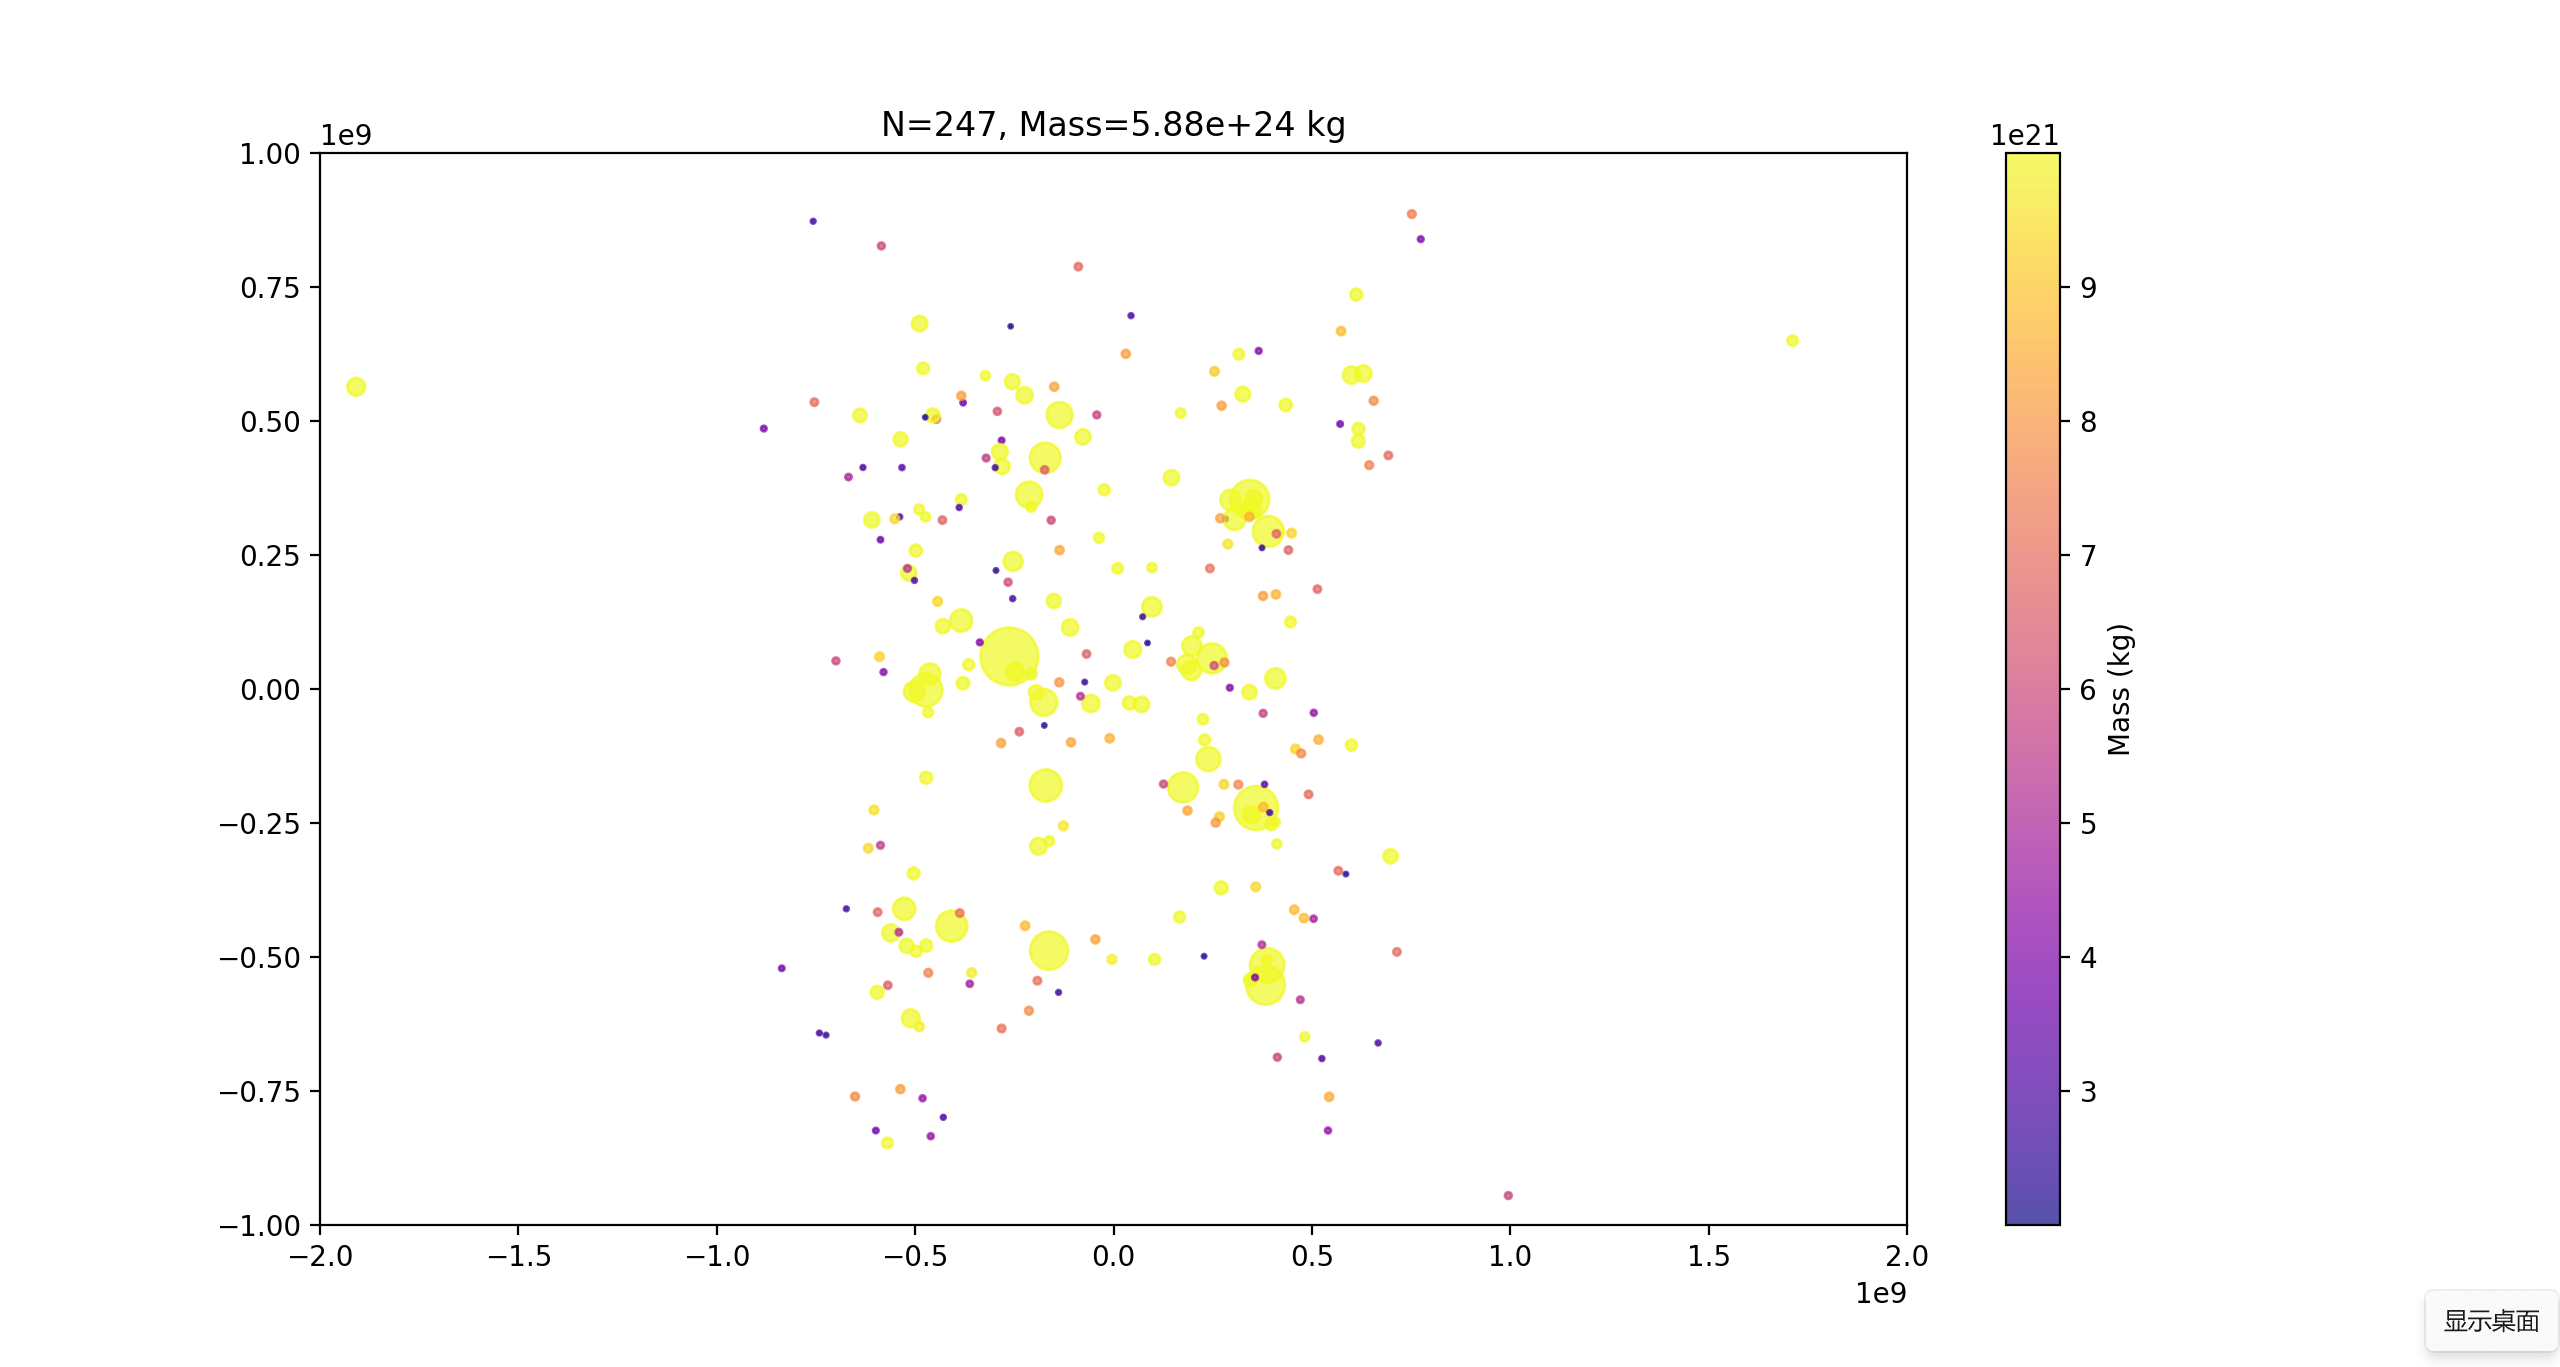
\includegraphics[width=0.48\linewidth]{images/247.png}}
    \subfigure[$N=148$]{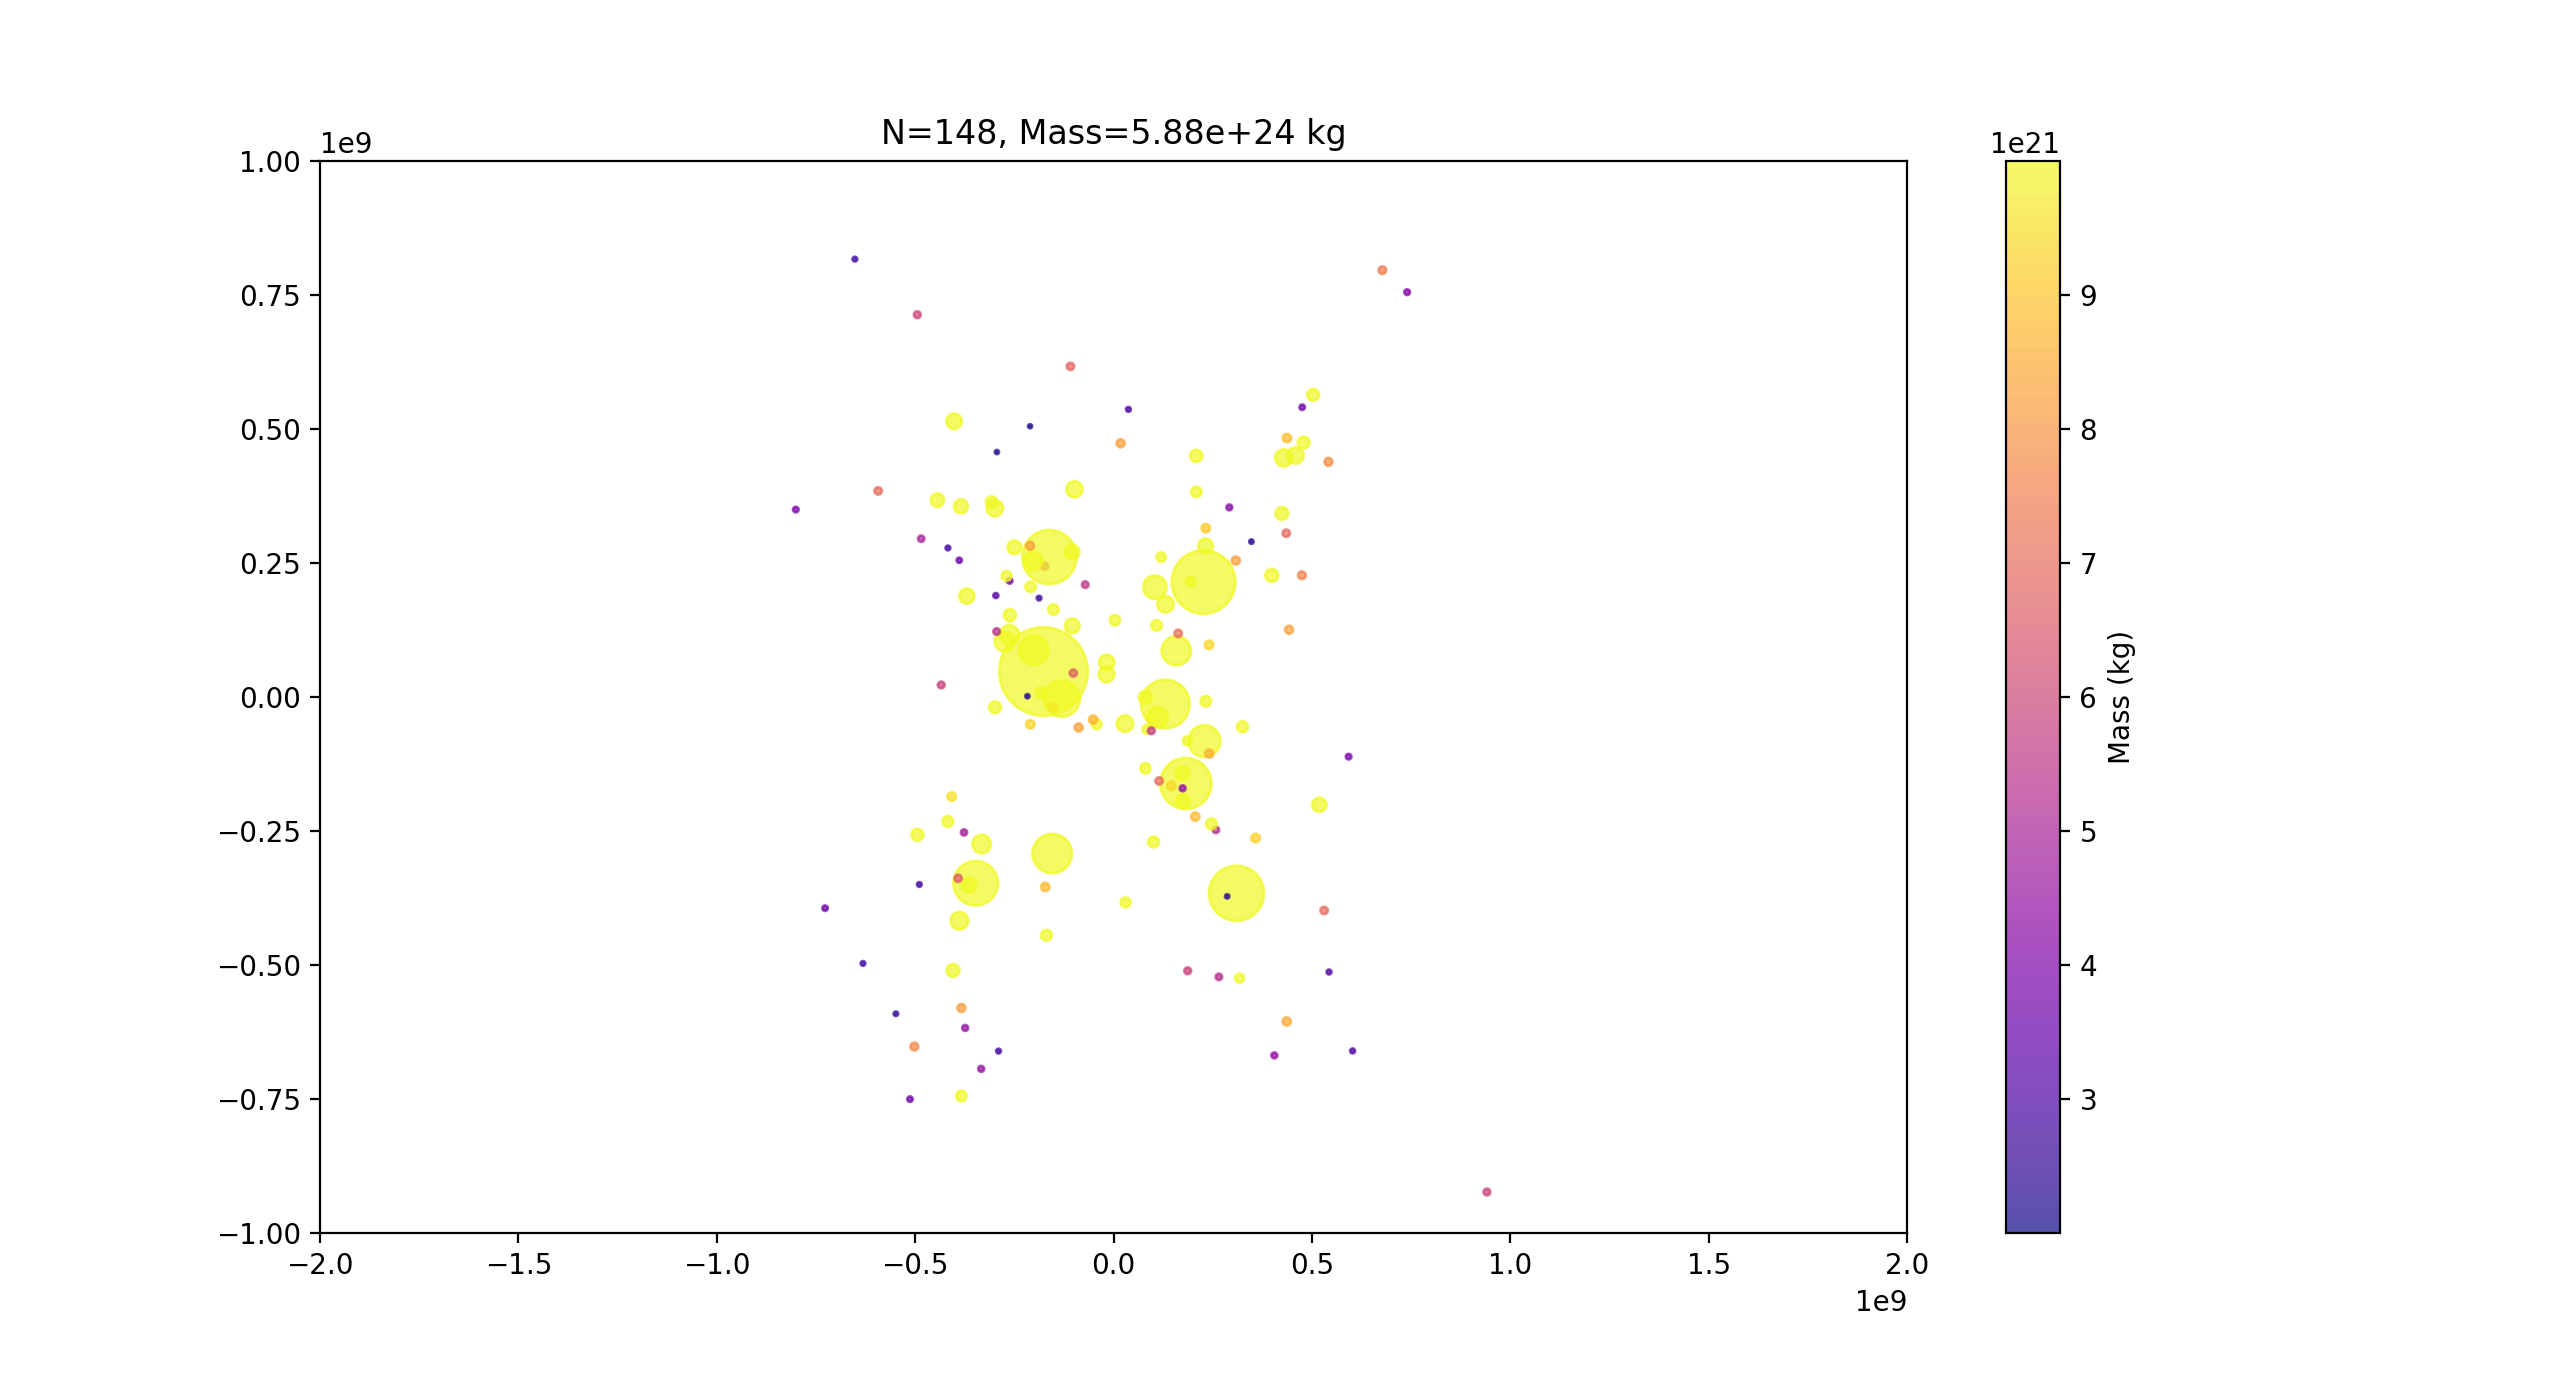
\includegraphics[width=0.48\linewidth]{images/148.png}}
    \subfigure[$N=82$]{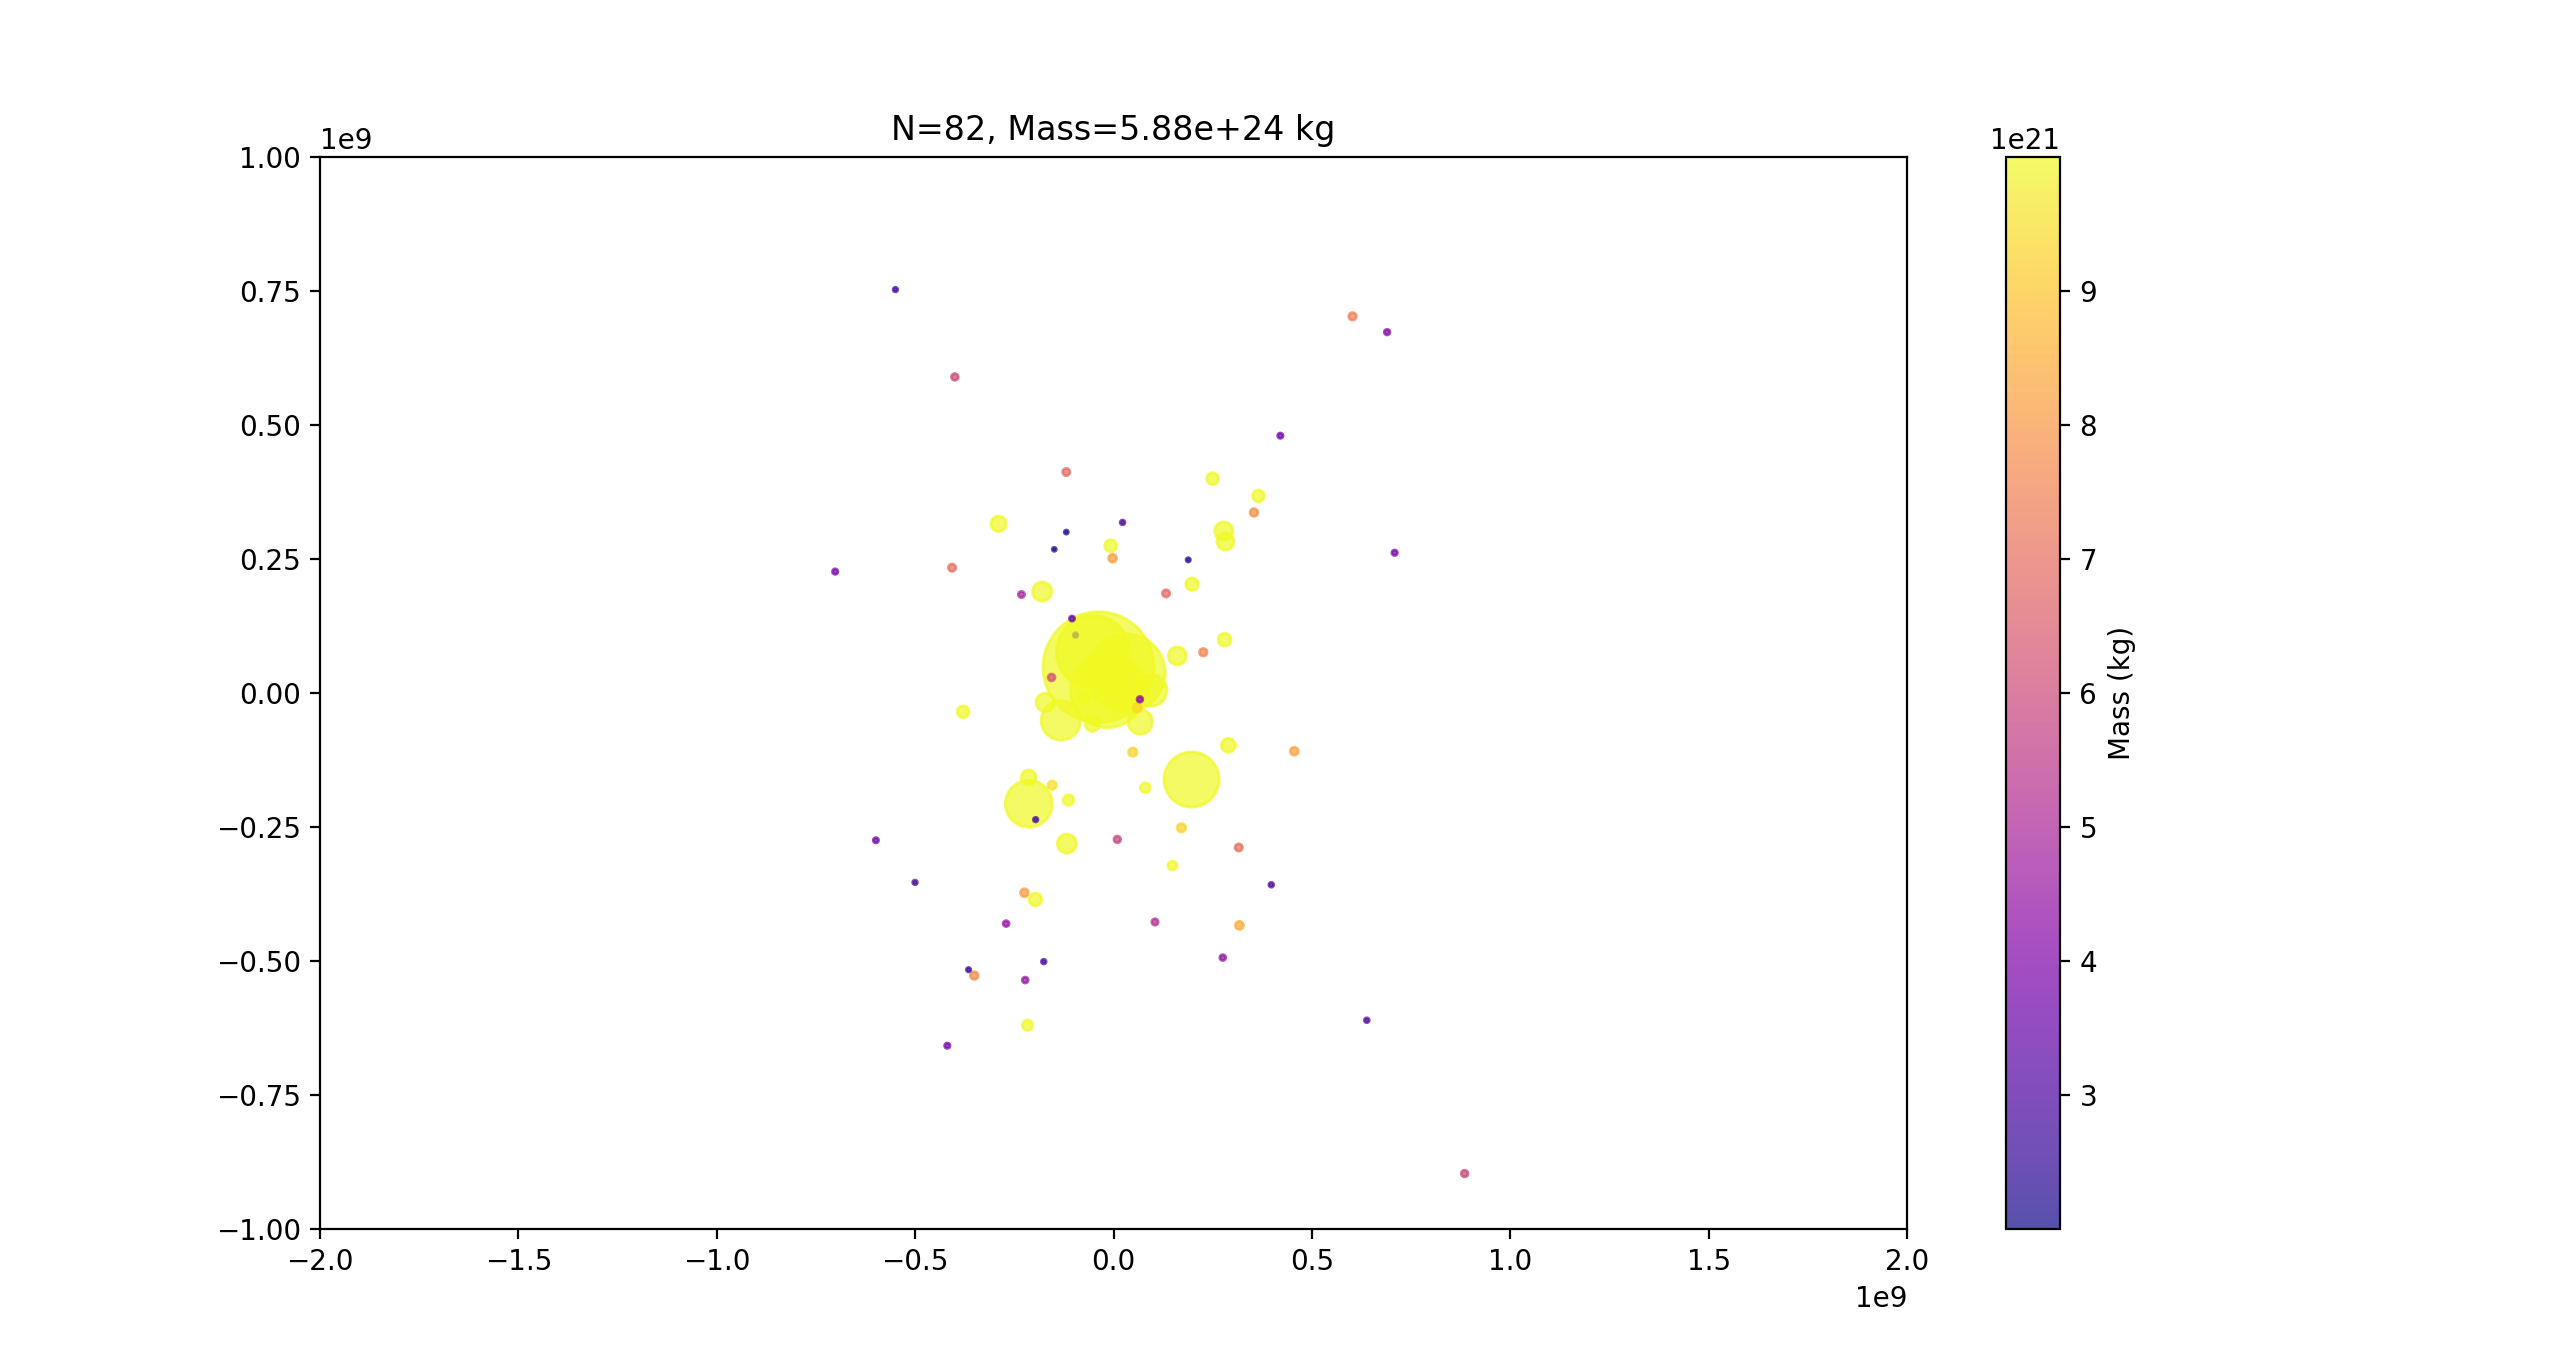
\includegraphics[width=0.48\linewidth]{images/82.png}}
    \subfigure[$N=49$]{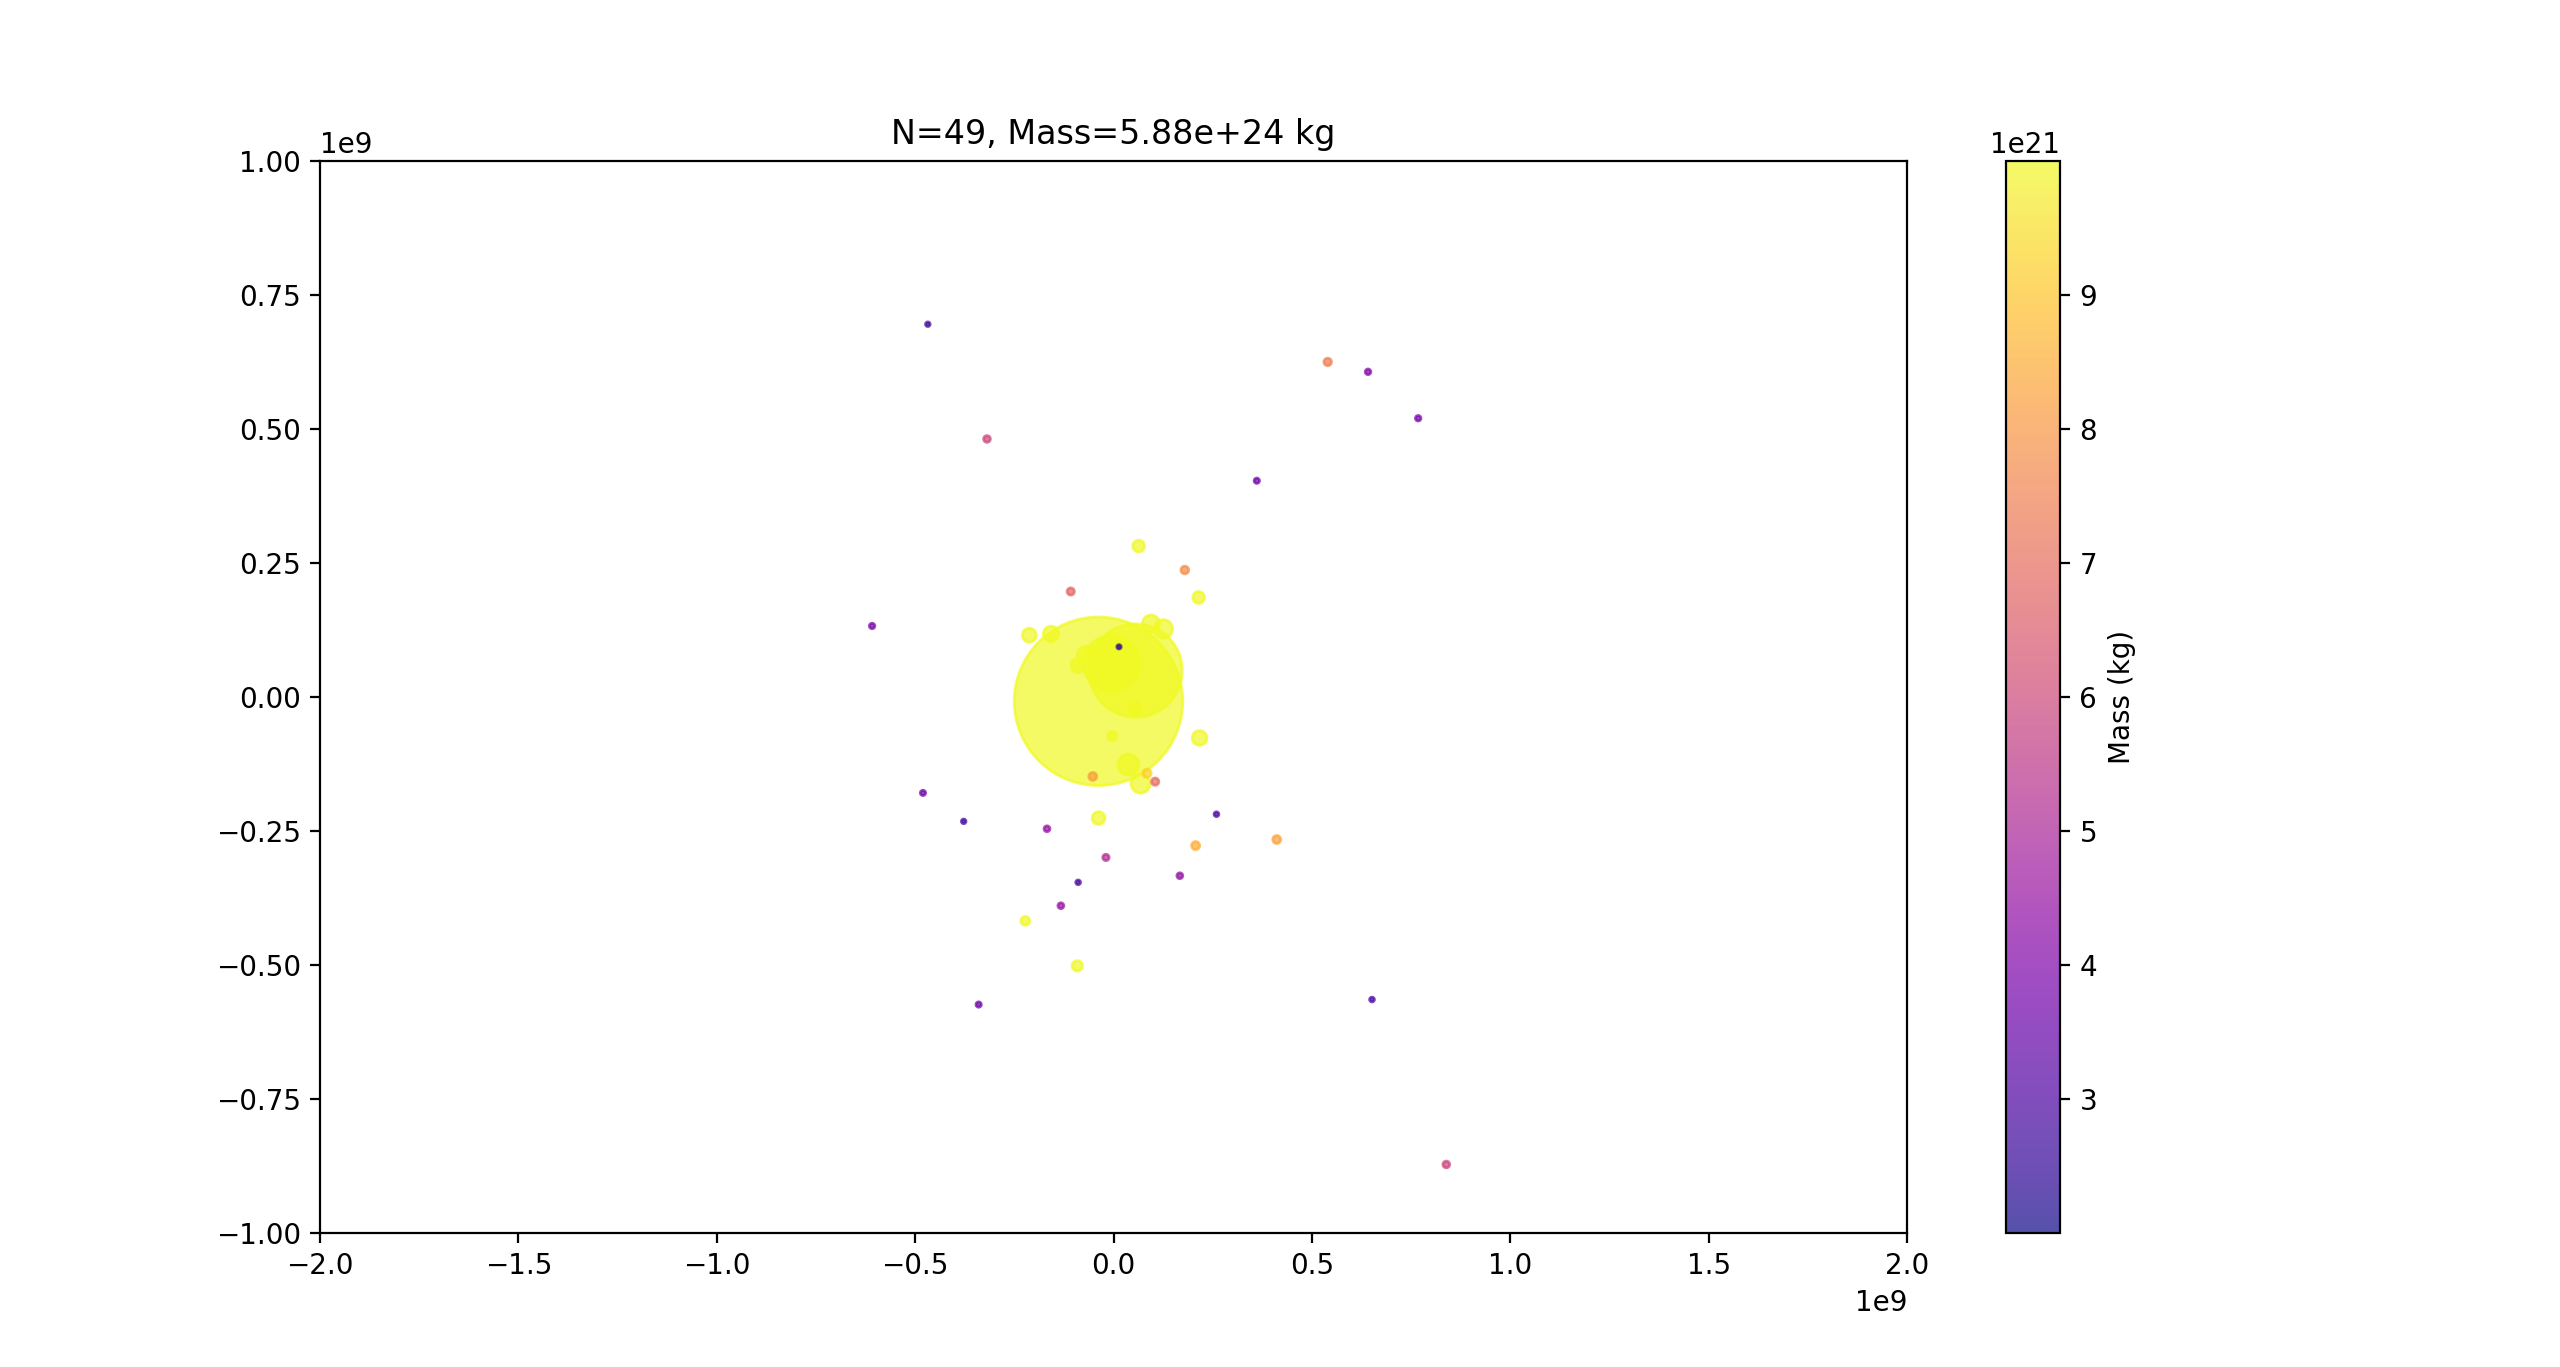
\includegraphics[width=0.48\linewidth]{images/49.png}}
    \subfigure[$N=16$]{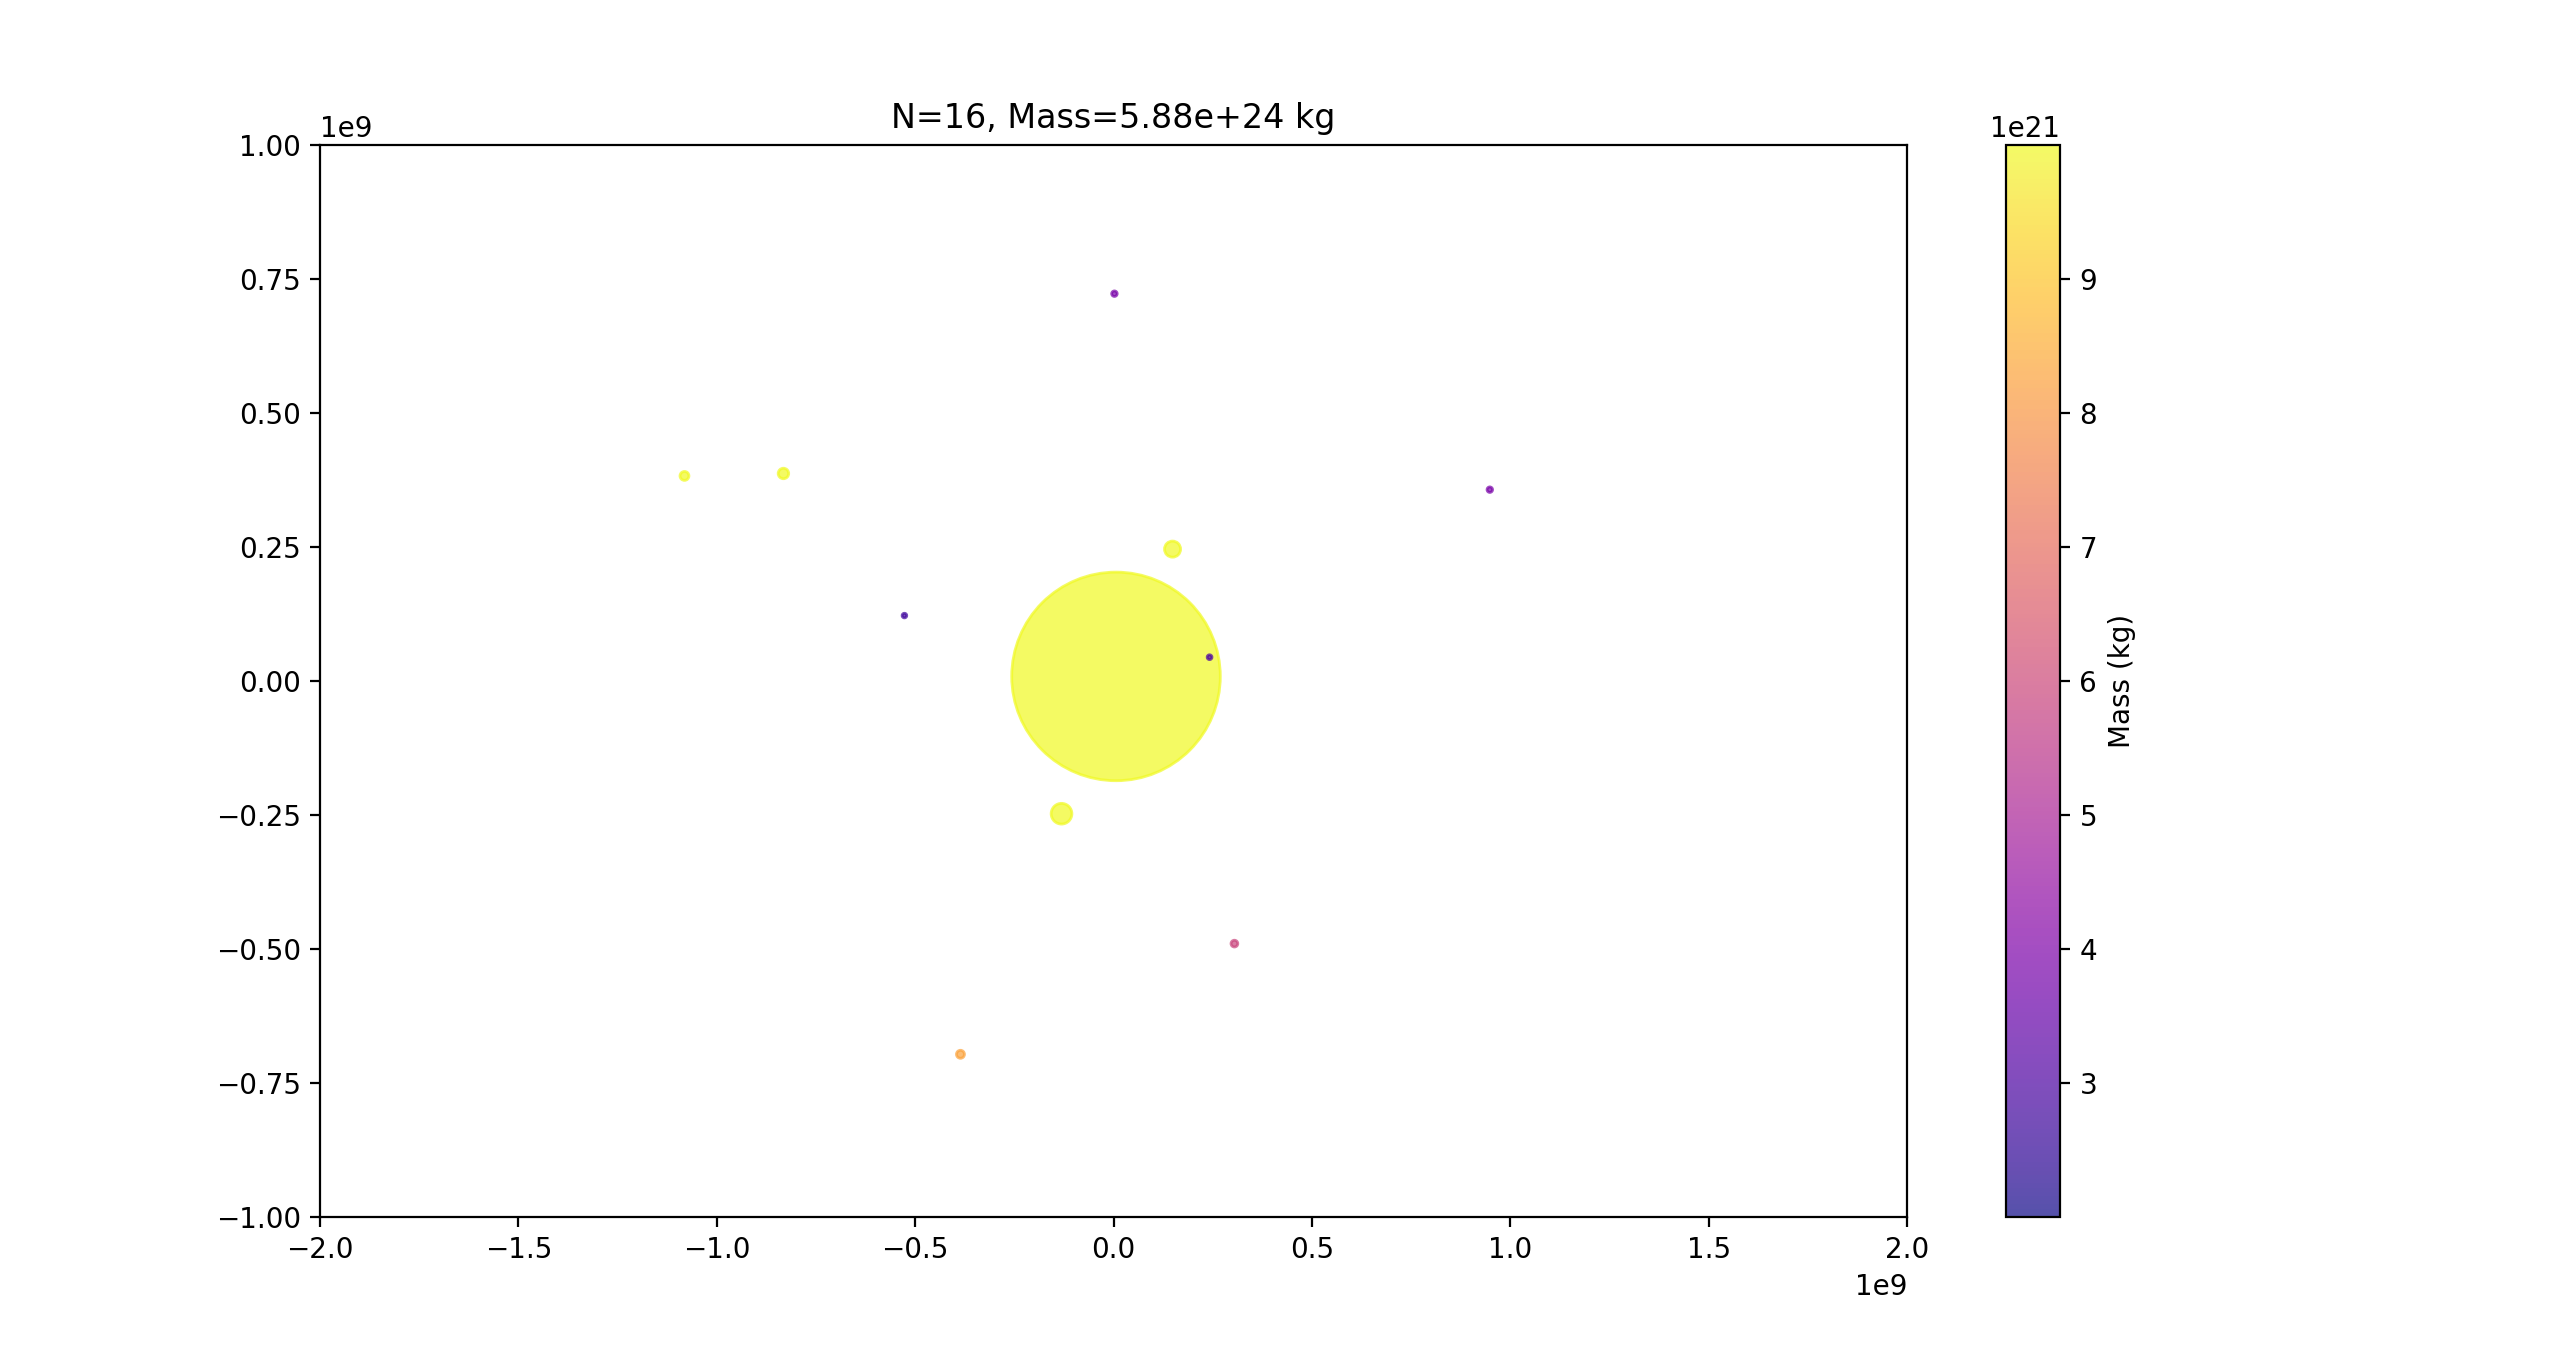
\includegraphics[width=0.48\linewidth]{images/16.png}}
    \caption{局域模拟结果示意图}
    \label{}
\end{figure}

这里设置模拟的区域大小为$10^9$km$\times$$10^9$km,边界如前面所介绍。需要注意的是,图中圆点的大小不代表粒子的半径,仅作为直观展示其质量的方式。
\subsection{分析与讨论}
合成的过程可以大致分为三个阶段:
\begin{itemize}
    \item \textbf{初步合并阶段:}在这一阶段,在模拟区域的各处相邻的小天体逐步合并为更大的天体,但是整体还是呈现出均匀分布的状态(图中的(a)(b)(c)部分);
    \item \textbf{核心形成阶段:}在这一阶段,一些较大的核心逐渐开始形成,分布在系统的各个位置,并开始吸引附近的粒子,持续增大(图中的(d)(e)(f)部分)
    \item \textbf{最终合并阶段:}在这一阶段,几乎全部合并的粒子向中心移动,并且合并为一个较大的天体,即为行星的初步形成,而周围的粒子绕其作圆周运动,成为小行星(若未被行星俘获)或者卫星(若被行星俘获)(图中的(g)(h)部分)。
\end{itemize}

\section{数值建模}

\section{实验结果}

\section{讨论}

\section{附录}

\end{document}
